% Chapter Template

% Main chapter title
%\chapter[toc version]{doc version}
\chapter{Domain generalization}

% Short version of the title for the header
%\chaptermark{version for header}

% Chapter Label
% For referencing this chapter elsewhere, use \ref{ChapterTemplate}
\label{chp:domain_generalization}

% Write text in here
% Use \subsection and \subsubsection to organize text

\begin{tcolorbox}
	\small{
		Some parts of this chapter were originally published in or adapted from:
		\begin{itemize}
			\item[] \cite{DeSIRe} \bibentry{DeSIRe} (presented in \Secref{sec:desire})
			\item[] \cite{AdvSInvConf} \bibentry{AdvSInvConf} (presented in \Secref{sec:adv_signer_inv})
			\item[] \cite{AdvSInvJournal} \bibentry{AdvSInvJournal} (idem)
			\item[] \cite{AdvInvAttack} \bibentry{AdvInvAttack} (\Secref{sec:adv_iris_attack})
		\end{itemize}

		The first two authors contributed equally in \cite{DeSIRe} and \cite{AdvSInvConf}. Both conceived the models and designed and conducted the experiments, with the supervision of Rebelo and Cardoso. Diogo Pernes was slightly more focused on the problem and model formalization, while Ferreira was more involved on dataset selection and preprocessing. The work in \cite{AdvSInvJournal} extends \cite{AdvSInvConf} by including a more exhaustive experimental evaluation. In \cite{AdvInvAttack}, Diogo Pernes contributed on the development of the proposed methodology, together with the first two authors, who motivated the application, formalized the problem and conducted all experiments. Rebelo and Cardoso supervised the work.
	}
\end{tcolorbox}

\section{Introduction}
\label{sec:chp4_intro}
In Chapters \ref{chp:networked_data_streams} and \ref{chp:domain_adaptation}, the target entities/domains were known at training time. In Chapter \ref{chp:networked_data_streams}, we exploited the correlations between different but related entities to augment the amount of data available for each of those and hence improve the in-distribution generalization. Chapter \ref{chp:domain_adaptation} was dedicated to the problem of domain adaptation, whose purpose is to improve the out-of-distribution (OOD) generalization in a specific target domain for which no labeled data is available.

In this chapter, we shall continue focusing on OOD generalization. However, now, the target domain is unknown and, therefore, no data from this domain is available at training time, neither labeled nor unlabeled. The purpose, then, is to use labeled data from multiple source domains to build a discriminative model that generalizes well to unknown OOD target domains -- a problem known as \emph{domain generalization} (\citet{Blanchard2011, Muandet2013}). Our main assumption to accomplish this goal is that the set of features that are relevant for the learning task are domain-invariant. Formally, we assume that, for each domain $\gD$, there exists a bijection $b_\gD: \gX \mapsto \gZ \times \gW$, where $\gZ$ is the domain-invariant space of features used for classification and $\gW$ are domain-specific auxiliary features carrying no relevant signal for the desired learning task. Thus, for $(\rz, \rw) \triangleq b_\gD(\rvx)$, we assume that $p_\gD(\ry \mid \rx) = p(\ry \mid \rz)$, i.e.\ the optimal classifier for any domain $\gD$ can be reconstructed from features in $\gZ$ and a domain-invariant classifier $p(\ry \mid \rz)$.  This formulation is closely related to the covariate shift assumption for domain adaptation, described in \Secref{sec:cov_shift_sota}.

A computer vision application where this problem is particularly relevant is sign language recognition (SLR). Large inter-signer variability in the manual signing process of sign languages is one of the challenges associated with this task. Due to this issue, models trained on data from a given set of signers often fail to generalize well when tested on previously unseen signers. Since, ideally, an SLR system should be able to recognize the gestures of any signer, this problem should be tackled with domain generalization (DG) techniques. For this reason, SLR will be the main application considered in this chapter. Nonetheless, we will also show that the same principles can be applied successfully to develop a fingerprint presentation attack detection method that exhibits robust performance on detecting unseen attacks.

The remainder of this chapter is organized as follows: i) we start by reviewing the state of the art for DG (\Secref{sec:dg_sota}); ii) we present a novel adversarial-based approach for DG in the context of SLR (\Secref{sec:adv_signer_inv}); iii) we show how this methodology can be successfully adapted to address the problem of iris presentation attack detection (\Secref{sec:adv_iris_attack}); iv) we present a novel reconstruction-based algorithm for DG (\Secref{sec:desire}).

\section{State of the art}
\label{sec:dg_sota}
\citet{Zhou2021} divide the algorithms for domain generalization as heterogeneous and homogeneous, depending on whether the label space varies (heterogeneous DG) or not (homogeneous DG). The former case is also known as \emph{zero-shot} domain generalization and its goal is, in general, to learn a feature representation that can be used in the target domain to recognize new classes. The latter, which will be the focus of this chapter, is closely related to domain adaptation, so there is a significant intersection between the two. \citet{Albuquerque2019} presented an upper bound for the generalization error that is essentially an upper bound for multi-source domain adaptation, similar to the bound by \citet{Zhao2018} (Theorem~\ref{thm:da_bound_multi_source}) and to our own (Theorem~\ref{thm:target_risk_bound}).

The theoretical proximity between the two problems motivates the existence of similar algorithms to tackle them. Many algorithms for DG actually follow the paradigm of domain alignment, which we have discussed extensively in the context of DA. \citet{Li2018} use an adversarial autoencoder and maximum mean discrepancy over its latent space to learn domain-invariant features. \citet{Ghifary2015} address the same problem through a multi-output autoencoder, which is trained to transform samples from one domain into samples from the remaining domains with the same label. \citet{Motiian2017} proposed a unified framework to address the problems of domain adaptation and generalization. They use a contrastive $\normltwo$-loss in the latent space that pushes together samples from different domains and the same class while pulling apart samples from different classes. Several other approaches extend the idea of domain adversarial networks (\citet{Ganin2015}) to the problem of domain generalization, by using domain classifiers and minimax training to learn domain-invariant features. Some of those use a single multi-class classifier to classify samples into one of $k$ source domains (e.g.\ \citet{Aslani2020, Matsuura2020}) and others employ $k$ binary domain discriminators trained in a one-vs-all manner (e.g.\ \citet{Shao2019, YaLi2018}).

Ensemble learning has also been widely applied to the problem of domain generalization. \citet{Zheng2014} train support vector machines (SVMs) with a single positive example and a few negative examples (known as \emph{exemplar-SVMs}) and use the most confident classifiers in an ensemble to make the final prediction. More recent approaches replace the SVM with deep neural networks and build ensembles of domain-specific networks, either by weighting all the predictions equally (e.g.\ \citet{Innocente2018, Zhou2020}) or by using the output of a domain classifier as sample-dependent ensemble weights (\citet{Wang2020a}).

Self-supervised learning (SSL) techniques are becoming increasingly popular in machine learning and have also been applied to the problem of DG. SSL refers to the task of learning from free labels, i.e.\ it consists of standard supervised pretraining on tasks where the labels can be extracted automatically from the data, without the need of manual annotation. Examples of SSL tasks are predicting the next word in a sentence, image colorization (\citet{Zhang2016}), predicting the relative position of image patches (\citet{Doersch2015}), predicting if a video is being played forward or backward (\citet{Wei2018}), etc. The idea motivating SSL is that the features learned by pretraining the model on self-supervised tasks provide good initializations for the model, which can then be finetuned for the desired task using a smaller amount of annotated data. In the scope of DG, SSL provides useful features regardless of the target task, reducing the overfitting to domain-specific biases (\citet{Zhou2021}). This idea was followed by \citet{Carlucci2019} and \citet{Wang2020b}, who trained a network to solve the Jigsaw puzzle (i.e.\ to place nine shuffled image patches back into their correct positions) as an auxiliary task to enhance domain generalization.

For a more complete review of DG theory and algorithms, please see \citet{Wang2021} and \citet{Zhou2021}.

\section{Adversarial domain generalization for signer-independent sign language recognition}
\label{sec:adv_signer_inv}

\subsection{Introduction}
Sign language is an integral form of communication and, currently, considered the standard education method of deaf people worldwide. It is a visual means of communication, with its own lexicon and grammar, that combines articulated hand gestures along with facial expressions to convey meaning. Deaf people have difficulty in speaking and learning spoken languages like hearing people. However, with sign language, they are able to communicate as efficiently and seamlessly. The population of sign language speakers is extended to family and friends of the deaf, interpreters, and those who learn the language by their own initiative. As most hearing people are unfamiliar with sign language, deaf people find it difficult to interact with the hearing majority. The result is the isolation of deaf communities from the overall society.

In this regard, automatically analyzing and recognizing sign language has become one of the key problems in the human computer-interaction field. SLR systems are meant to automatically translate signs into the corresponding text or speech. This is important not only to bridge the communication gap between deaf and hearing people but also to increase the amount of content the deaf can access, such as the creation of educational tools or games for deaf people and visual dictionaries of sign language.

The SLR problem has been addressed in the literature by means of wearable devices (e.g.\ data gloves or similar equipments) or vision-based systems (\citet{Ahdal2012}). Vision-based systems, either those using color or depth information, face the problem of the inherently noisy and ambiguous nature of the input data. Data gloves yield more reliable and descriptive features. Nevertheless, vision-based SLR systems are arguably the most natural choice for real-world applications. Vision-based SLR is less invasive since there is no need to wear cumbersome devices that may affect the natural signing movement.

Several vision-based SLR methodologies have been proposed over the last twenty years, with increasing progress in the recognition performance. An important part of this recent progress was achieved thanks to the emergence of deep learning approaches and more specifically with CNNs (\citet{Pigou2015, Koller2016, Wu2016, Neverova2016, Kumar2017}).

A practical SLR system must operate in a signer-independent scenario. That is, the signer of the probe must not be seen during the training process of the models. Although current SLR systems demonstrate excellent performance for signer-dependent settings, their recognition rates typically decrease significantly when the signer is new to the system. This performance drop is the result of the large inter-signer variability in the manual signing process of sign languages.

Although the appearance of manual signs is well-defined in sign language dictionaries, in practice, variations may arise due to regional and social factors, and also from age, gender, education and family background. This can lead to significant variations in manual signs performed by different signers, and pose challenging problems for developing robust signer-independent SLR systems. \Figref{fig:inter_signer_variations} illustrates inter-signer variability by showing six different signers performing the same gestures.

\begin{figure}[t]
    \centering
    \subfloat{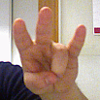
\includegraphics[width=0.15\textwidth]{ChapterFour/1.png}}
    \hfill
    \subfloat{
\includegraphics[width=0.15\textwidth]{ChapterFour/4.png}}
    \hfill
    \subfloat{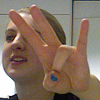
\includegraphics[width=0.15\textwidth]{ChapterFour/3.png}}
    \\\vspace{0.4cm}
    \subfloat{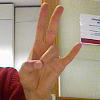
\includegraphics[width=0.15\textwidth]{ChapterFour/2.png}}
    \hfill
    \subfloat{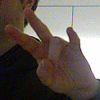
\includegraphics[width=0.15\textwidth]{ChapterFour/5.png}}
    \hfill
    \subfloat{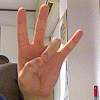
\includegraphics[width=0.15\textwidth]{ChapterFour/6.png}}
    \caption{Inter-signer variability: it is possible to observe not only phonological variations (e.g.\ different handshapes, palm orientations, and sign locations) but also a large physical variability (e.g.\ different hand sizes) when six signers are performing the same sign.}
    \label{fig:inter_signer_variations}
\end{figure}

Borrowing from recent works on adversarial neural networks (\citet{Goodfellow2014, Feutry2018}) and domain transfer (\citet{Ganin2015}), we introduce a deep neural network along with a novel adversarial training objective to specifically tackle the signer-independent SLR problem. The underlying idea is to preserve as much information as possible about the signs, while discarding the signer-specific information that is implicitly present in the manual signing process. For this purpose, the proposed deep model is composed by an \emph{encoder} network, which maps from the input images to latent representations, as well as two discriminative classifiers operating on top of these underlying representations, namely the \emph{sign-classifier} network and the \emph{signer-classifier} network. While the former is trained to predict the sign labels, the latter is trained to identify the signer. In addition, the parameters of the encoder network are optimized to minimize the loss of the sign-classifier while trying to fool the signer-classifier network. This adversarial and competitive training scheme encourages the learned representations to be signer-invariant and highly discriminative for the sign classification task. To further constrain the latent representations to be signer-invariant, we introduce an additional training objective that operates on the hidden representations of the encoder network in order to enforce the latent distributions of different signers to be as similar as possible.

Although this adversarial training framework is similar to those initially introduced by \citet{Ganin2015}, in the context of domain adaptation, and then by \citet{Feutry2018} to learn anonymized representations, our main contributions on top of these works are two-fold: i) the application of the adversarial training concept to the signer-independent SLR problem and ii) a novel adversarial training objective that differs from the ones of \citet{Ganin2015} and \citet{Feutry2018} in two ways. First, our training objective is minimum if and only if the adversarial classifier (i.e.\ the signer-classifier) produces a uniform distribution over the domains (i.e.\ signer identities). Second, we introduce an additional term to the adversarial training objective that further discourages the learned representations of retaining any signer-specific information, by explicitly imposing similarity in the latent distributions of different signers.

The remainder of this section is organized as follows. \Secref{sec:adv_signer_inv_rel_work} presents the related work on SLR. The proposed model along with its adversarial training scheme are fully described in \Secref{sec:adv_signer_inv_method}. Experimental results and conclusions are reported in Sections~\ref{sec:adv_signer_inv_experiments} and \ref{sec:adv_signer_inv_conclusion}, respectively.

\subsection{Related Work}
\label{sec:adv_signer_inv_rel_work}
We have discussed some of the most relevant approaches for DG in \Secref{sec:dg_sota}, so now we shall focus our attention on the specific problem of SLR. This has become an appealing topic in modern society because such systems can ideally be used to reduce the communication barriers that exist between deaf and hearing people.
SLR approaches can be broadly divided into: (i) isolated, which address the recognition of single signs either using static images or video (\citet{Marin2014, Marin2016}), and (ii) continuous, which correspond to the recognition of sentences represented as a sequence of signs (\citet{DanGuo2017, DanGuo2018, Wang2018}). Although most recent works focus on the continuous SLR and its associated problems (e.g.\ large vocabulary size), static SLR is still a challenging task, especially under unconstrained scenarios. One of the biggest challenges is related to the large inter-signer variability, which is in fact the focus of this work.

According to the amount of data required from the test signers, previously signer-independent SLR works can be broadly divided into two main groups: (i) signer adaptation approaches, where a previous trained model is adapted to a new signer by using a small amount of signer specific data, and (ii) truly signer independent methodologies, in which a generic model robust for new test signers is built without using data of those test signers.

The former signer adaptation approaches were greatly inspired by speaker adaptation methods from the speech recognition research. \citet{Agris2006} used maximum likelihood linear regression (MLLR) and maximum a posteriori (MAP) estimation for signer adaptation. In a subsequent work (\citet{Agris2008a}), they extended their work by combining the eigenvoice approach by \citet{Kuhn2000} with MLLR and MAP to adapt trained hidden Markov models (HMMs) to new signers. MLLR and MAP were the basic adaptation strategies, and the eigenvoice approach provided constraints to reduce the number of free parameters to be adapted. More recently, \citet{Kim2016} investigated the potential of several signer normalization techniques (e.g.\ speed normalization) and different deep neural network adaptation strategies for the signer-independence problem. They found that while signer normalization is ineffective, a simple neural network adaptation strategy, such as fine-tuning the signer-specific neural networks on the adaptation data, is very effective.

The aforementioned methods are all supervised adaptation approaches, in the sense that the adaptation data from the new signer must be labeled. However, in practice, collecting labeled data may be a cumbersome and time-consuming task. To overcome this issue, a few works have resorted to unsupervised adaptation strategies. \citet{Yin2015} proposed a two-step weakly supervised metric learning framework to perform signer adaptation with some unlabeled sign data of the new signer. In the first step, a generic metric is learnt from the available labeled data of several different signers. In the second step, the generic metric is adapted to the new signer by considering clustering and manifold constraints along with the collected unlabeled data.

Although signer adaptation is a reasonable approach, there is still the need to collect either labeled or unlabeled data to retrain and adapt the model to a new signer. Therefore, a truly signer-independent approach, which does not require any data from the new signers, would be the ideal solution for a practical SLR system. Examples of such works can be found are those by \citet{Zieren2005, Shanableh2011, Agris2008b, Kong2014, Kelly2010, Dahmani2014, Yin2016}. Most of them involved a huge feature engineering effort in order to build normalized feature descriptors robust to the physical variations of the signers (e.g.\ height, hand size and length of the arm) and different acquisition conditions (e.g.\ distance to the camera). Afterwards, most of these works use HMMs or their variants for sign recognition. It is the example of the work proposed by \citet{Agris2008b}, in which a set of 11 regional features are extracted (e.g.\ 2-D coordinates, hand blobs area, orientation of the main axis, inertia ratio, eccentricity and compactness) and then normalized according to the head position and shoulders distance of the signer. \citet{Kelly2010} introduced a novel signer-independent hand posture feature descriptor, along with an eigenspace size function which represents both qualitative and quantitative properties of a visual shape. \citet{Kong2014} gave particular importance to the movement of epenthesis (ME), which appears as the transition movement that connects successive signs. Concretely speaking, they removed the ME by using a segment and merge approach to decrease the inter-signer variations in ME and used a two-layer conditional random field classifier for sign recognition. More recently, \citet{Yin2016} proposed an interesting and alternative approach that relies on distance metric learning. In particular, the metric is learnt by constraining the distances between the training samples and generic references of the sign classes. The references are constructed by signer invariant representations of each sign class (i.e.\ the average of all samples within the specific class). Afterwards, a two-step iterative optimization strategy is employed to obtain more appropriate references and update the corresponding distance metric alternately.

Although the aforementioned methods have promoted a significant evolution in the signer-independent research, there are still many opportunities for improvement. A major weakness across all the methods is related to the fact that representation and metric learning are not performed jointly. It is well known that the recent success of deep learning approaches, particularly those using CNNs, in tasks like object detection and recognition, has been extended to the SLR problem. The underlying motivation is to automatically learn multiple levels of representations directly from the data (\citet{Pigou2015, Koller2016, Wu2016, Neverova2016, Kumar2017}). However, none of these explicitly constrains the learned representations to be signer invariant.

\subsection{Methodology}
\label{sec:adv_signer_inv_method}

The ultimate goal of our model is to learn signer-invariant latent representations that preserve the relevant part of the information about the signs while discarding the signer-specific traits that may hamper the sign classification task. To accomplish this purpose, we introduce a deep neural network along with an adversarial training scheme that is able to learn feature representations that combine both sign discriminativeness and signer-invariance.

More specifically, let $\{(\mX_{i},y_{i},s_{i})\}_{i=1}^{n}$ be a labeled dataset of $n$ samples, where $\mX_{i}$ represents the $i$-th colour image, and $y_{i} \in \gY$ and $s_{i} \in \{1,2,\dots,k\}$ denote the corresponding class (sign) label and signer identity, respectively. To induce the model to learn signer-invariant representations, the proposed model comprises three distinct sub-networks:
\begin{itemize}
    \item an encoder network, which aims at learning an encoding function $g(\cdot;\vtheta_g): \gX \mapsto \gZ$, parameterized by $\vtheta_g$, that maps from an input image $\mX \in \gX$ to a latent representation $\vz \in \gZ$;
    \item a sign-classifier network, which operates on top of this underlying latent representation $\vz$ to learn our task-specific function $h(\cdot; \vtheta_h): \gZ \mapsto \gY$, parameterized by $\vtheta_h$, that maps latent vectors into the predicted probabilities of each sign class;
    \item a signer-classifier network, with the purpose of learning a signer-specific function $d(\cdot; \vtheta_d): \gZ \mapsto \{1,2,\dots,k\}$, parameterized by $\vtheta_d$, that maps the same hidden representation $\vz$ into the corresponding signer identity.
\end{itemize}

During the learning stage, the parameters of both classifiers are optimized in order to minimize their errors on their specific tasks on the training set. In addition, the parameters of the encoder network are optimized in order to minimize the loss of the sign-classifier network while forcing the signer-classifier to be a random guessing predictor. In the course of this adversarial training procedure, the learned latent representations $\vz$ are encouraged to be signer-invariant and highly discriminative for sign classification. To further discourage the latent representations of retaining any signer-specific traits, we introduce an additional training objective that enforces the latent distributions of different signers to be as similar as possible.

\subsubsection{Architecture}
As illustrated in \Figref{fig:model_archi}, the architecture of the proposed model is composed by three main sub-networks or blocks, i.e. an encoder, a sign-classifier, and a signer-classifier.

The encoder network attempts to learn a mapping from an input image $\mX$ to a latent representation $\vz$. It consists of a sequence of three pairs of consecutive $3\times 3$ convolutional layers with Rectified  Linear  Units (ReLUs) as non-linearities. For downsampling, the last convolutional layer of each pair has a stride of 2. The number of filters starts as 32 and is doubled after each convolutional pair. The dense layer on top of the encoder network has 128 neurons. On top of that, there is a fully-connected layer, also with a ReLU, outputting the desired signer-invariant latent representations $\vz$.

Taking the latent representations $\vz$ as input, the sign-classifier block is composed by a sequence of three fully-connected layers, with ReLUs as the non-linear functions, for predicting the sign class $\hat{y} \triangleq h(\vz; \vtheta_h)$. The number of nodes of each hidden layer was set to 128. The last fully-connected layer has a softmax activation function which outputs the probabilities for each sign class.

The signer-classifier network has exactly the same topology as the sign-classifier. However, it maps the latent representations $\vz$ to the predicted signer identity $\hat{s} \triangleq d(\vz; \vtheta_d)$. Therefore, the number of nodes of the output layer equals the number of signers in the training set.


\begin{figure*}[t]
\centering
\tikzset{every picture/.style={line width=0.75pt}} %set default line width to 0.75pt

\scalebox{0.6}{










\tikzset{every picture/.style={line width=0.9pt}} %set default line width to 0.75pt

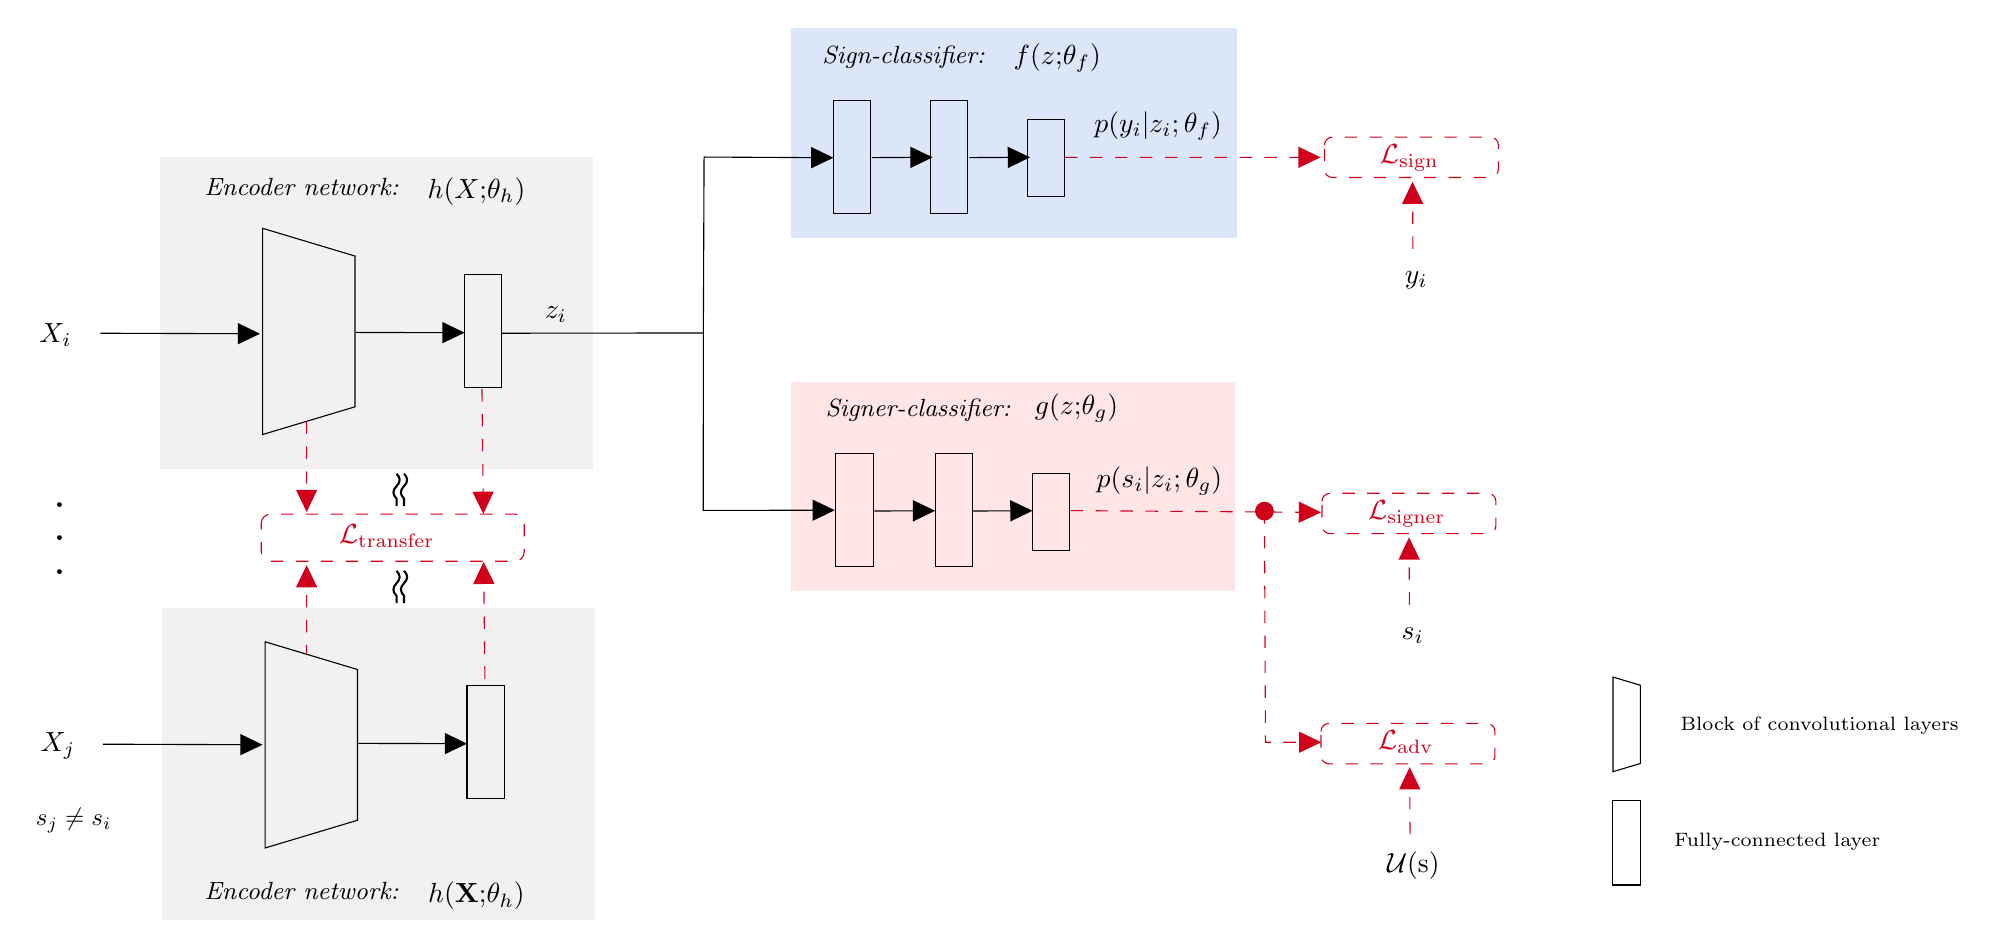
\begin{tikzpicture}[x=0.9pt,y=0.9pt,yscale=-1,xscale=1]
%uncomment if require: \path (0,637); %set diagram left start at 0, and has height of 637

%Shape: Rectangle [id:dp7817430644997849]
\draw  [draw opacity=0][fill={rgb, 255:red, 226; green, 223; blue, 223 }  ,fill opacity=0.46 ][dash pattern={on 4.5pt off 4.5pt}] (89.57,241.83) -- (263.45,241.83) -- (263.45,367) -- (89.57,367) -- cycle ;
%Shape: Rectangle [id:dp43448545781433445]
\draw  [draw opacity=0][fill={rgb, 255:red, 124; green, 163; blue, 233 }  ,fill opacity=0.27 ][dash pattern={on 4.5pt off 4.5pt}] (342,9) -- (521,9) -- (521,93.23) -- (342,93.23) -- cycle ;
%Shape: Rectangle [id:dp47448290384115754]
\draw  [draw opacity=0][fill={rgb, 255:red, 226; green, 223; blue, 223 }  ,fill opacity=0.46 ][dash pattern={on 4.5pt off 4.5pt}] (88.57,60.83) -- (262.45,60.83) -- (262.45,186) -- (88.57,186) -- cycle ;
%Shape: Trapezoid [id:dp7544890433922595]
\draw   (129.83,89.34) -- (166.92,100.47) -- (166.92,161) -- (129.83,172.13) -- cycle ;
%Shape: Rectangle [id:dp07852532899632947]
\draw   (225.83,108) -- (225.83,153.36) -- (210.91,153.36) -- (210.91,108) -- cycle ;
%Straight Lines [id:da6483299081027241]
\draw    (167.27,131.14) -- (208.91,131.24) ;
\draw [shift={(210.91,131.24)}, rotate = 180.14] [fill={rgb, 255:red, 0; green, 0; blue, 0 }  ][line width=0.75]  [draw opacity=0] (8.93,-4.29) -- (0,0) -- (8.93,4.29) -- cycle    ;

%Straight Lines [id:da3383332186453154]
\draw    (64.69,131.46) -- (126.8,131.67) ;
\draw [shift={(128.8,131.68)}, rotate = 180.19] [fill={rgb, 255:red, 0; green, 0; blue, 0 }  ][line width=0.75]  [draw opacity=0] (8.93,-4.29) -- (0,0) -- (8.93,4.29) -- cycle    ;

%Straight Lines [id:da8976159443553993]
\draw    (225.86,131.46) -- (306.79,131.35) ;


%Shape: Rectangle [id:dp39844785350453726]
\draw   (373.93,38.03) -- (373.93,83.38) -- (359.01,83.38) -- (359.01,38.03) -- cycle ;
%Shape: Rectangle [id:dp5960148926786581]
\draw   (412.75,38.03) -- (412.75,83.38) -- (397.84,83.38) -- (397.84,38.03) -- cycle ;
%Shape: Rectangle [id:dp2968748699957451]
\draw   (451.86,45.72) -- (451.86,76.69) -- (436.94,76.69) -- (436.94,45.72) -- cycle ;
%Straight Lines [id:da38135442637321804]
\draw    (374.47,60.94) -- (396.84,60.84) ;
\draw [shift={(398.84,60.83)}, rotate = 539.75] [fill={rgb, 255:red, 0; green, 0; blue, 0 }  ][line width=0.75]  [draw opacity=0] (8.93,-4.29) -- (0,0) -- (8.93,4.29) -- cycle    ;

%Straight Lines [id:da5103446228646831]
\draw    (413.57,60.94) -- (435.94,60.84) ;
\draw [shift={(437.94,60.83)}, rotate = 539.75] [fill={rgb, 255:red, 0; green, 0; blue, 0 }  ][line width=0.75]  [draw opacity=0] (8.93,-4.29) -- (0,0) -- (8.93,4.29) -- cycle    ;

%Shape: Rectangle [id:dp21504155648063916]
\draw  [draw opacity=0][fill={rgb, 255:red, 255; green, 199; blue, 199 }  ,fill opacity=0.46 ][dash pattern={on 4.5pt off 4.5pt}] (342.06,150.9) -- (520.25,150.9) -- (520.25,235.13) -- (342.06,235.13) -- cycle ;
%Shape: Rectangle [id:dp5629086137047858]
\draw   (374.93,179.92) -- (374.93,225.28) -- (360.01,225.28) -- (360.01,179.92) -- cycle ;
%Shape: Rectangle [id:dp11383387176162141]
\draw   (414.75,179.92) -- (414.75,225.28) -- (399.84,225.28) -- (399.84,179.92) -- cycle ;
%Shape: Rectangle [id:dp8834314863600405]
\draw   (453.86,187.61) -- (453.86,218.59) -- (438.94,218.59) -- (438.94,187.61) -- cycle ;
%Straight Lines [id:da7960584409422926]
\draw    (375.47,202.84) -- (397.84,202.74) ;
\draw [shift={(399.84,202.73)}, rotate = 539.75] [fill={rgb, 255:red, 0; green, 0; blue, 0 }  ][line width=0.75]  [draw opacity=0] (8.93,-4.29) -- (0,0) -- (8.93,4.29) -- cycle    ;

%Straight Lines [id:da26603179330471005]
\draw    (414.57,202.84) -- (436.94,202.74) ;
\draw [shift={(438.94,202.73)}, rotate = 539.75] [fill={rgb, 255:red, 0; green, 0; blue, 0 }  ][line width=0.75]  [draw opacity=0] (8.93,-4.29) -- (0,0) -- (8.93,4.29) -- cycle    ;

%Straight Lines [id:da645470302869213]
\draw    (306.79,131.35) -- (307.07,60.72) -- (357,60.99) ;
\draw [shift={(359,61)}, rotate = 180.31] [fill={rgb, 255:red, 0; green, 0; blue, 0 }  ][line width=0.75]  [draw opacity=0] (8.93,-4.29) -- (0,0) -- (8.93,4.29) -- cycle    ;

%Straight Lines [id:da6326177139350364]
\draw    (306.79,131.35) -- (306.74,202.61) -- (357.56,202.5) ;
\draw [shift={(359.56,202.5)}, rotate = 539.88] [fill={rgb, 255:red, 0; green, 0; blue, 0 }  ][line width=0.75]  [draw opacity=0] (8.93,-4.29) -- (0,0) -- (8.93,4.29) -- cycle    ;

%Straight Lines [id:da43094599217232044]
\draw [color={rgb, 255:red, 208; green, 2; blue, 27 }  ,draw opacity=1 ] [dash pattern={on 4.5pt off 4.5pt}]  (452.06,60.88) -- (552.61,60.84) ;
\draw [shift={(554.61,60.83)}, rotate = 539.98] [fill={rgb, 255:red, 208; green, 2; blue, 27 }  ,fill opacity=1 ][line width=0.75]  [draw opacity=0] (8.93,-4.29) -- (0,0) -- (8.93,4.29) -- cycle    ;

%Rounded Rect [id:dp20102262667247417]
\draw  [color={rgb, 255:red, 208; green, 2; blue, 27 }  ,draw opacity=1 ][dash pattern={on 4.5pt off 4.5pt}] (555.16,198.96) .. controls (555.16,197.16) and (556.62,195.71) .. (558.41,195.71) -- (621.75,195.71) .. controls (623.55,195.71) and (625,197.16) .. (625,198.96) -- (625,208.69) .. controls (625,210.48) and (623.55,211.94) .. (621.75,211.94) -- (558.41,211.94) .. controls (556.62,211.94) and (555.16,210.48) .. (555.16,208.69) -- cycle ;
%Straight Lines [id:da7107772326187543]
\draw [color={rgb, 255:red, 208; green, 2; blue, 27 }  ,draw opacity=1 ] [dash pattern={on 4.5pt off 4.5pt}]  (454.25,202.67) -- (552.78,203.37) ;
\draw [shift={(554.78,203.38)}, rotate = 180.41] [fill={rgb, 255:red, 208; green, 2; blue, 27 }  ,fill opacity=1 ][line width=0.75]  [draw opacity=0] (8.93,-4.29) -- (0,0) -- (8.93,4.29) -- cycle    ;

%Straight Lines [id:da7856916848123423]
\draw [color={rgb, 255:red, 208; green, 2; blue, 27 }  ,draw opacity=1 ] [dash pattern={on 4.5pt off 4.5pt}]  (147.5,166.88) -- (147.51,201.24) ;
\draw [shift={(147.51,203.24)}, rotate = 269.99] [fill={rgb, 255:red, 208; green, 2; blue, 27 }  ,fill opacity=1 ][line width=0.75]  [draw opacity=0] (8.93,-4.29) -- (0,0) -- (8.93,4.29) -- cycle    ;

%Straight Lines [id:da899109719860808]
\draw [color={rgb, 255:red, 208; green, 2; blue, 27 }  ,draw opacity=1 ] [dash pattern={on 4.5pt off 4.5pt}]  (217.9,153.87) -- (218.43,202) ;
\draw [shift={(218.45,204)}, rotate = 269.36] [fill={rgb, 255:red, 208; green, 2; blue, 27 }  ,fill opacity=1 ][line width=0.75]  [draw opacity=0] (8.93,-4.29) -- (0,0) -- (8.93,4.29) -- cycle    ;

%Straight Lines [id:da36002582240035363]
\draw [color={rgb, 255:red, 0; green, 0; blue, 0 }  ,draw opacity=1 ][line width=0.75]    (186.6,226.85) .. controls (188.27,228.52) and (188.27,230.18) .. (186.6,231.85) .. controls (184.93,233.52) and (184.93,235.18) .. (186.6,236.85) -- (186.6,239.85) -- (186.6,239.85)(183.6,226.85) .. controls (185.27,228.52) and (185.27,230.18) .. (183.6,231.85) .. controls (181.93,233.52) and (181.93,235.18) .. (183.6,236.85) -- (183.6,239.85) -- (183.6,239.85) ;


%Rounded Rect [id:dp28118263286951617]
\draw  [color={rgb, 255:red, 208; green, 2; blue, 27 }  ,draw opacity=1 ][dash pattern={on 4.5pt off 4.5pt}] (556.16,55.96) .. controls (556.16,54.16) and (557.62,52.71) .. (559.41,52.71) -- (622.75,52.71) .. controls (624.55,52.71) and (626,54.16) .. (626,55.96) -- (626,65.69) .. controls (626,67.48) and (624.55,68.94) .. (622.75,68.94) -- (559.41,68.94) .. controls (557.62,68.94) and (556.16,67.48) .. (556.16,65.69) -- cycle ;
%Straight Lines [id:da5356763271282314]
\draw [color={rgb, 255:red, 208; green, 2; blue, 27 }  ,draw opacity=1 ] [dash pattern={on 4.5pt off 4.5pt}]  (591.52,72.62) -- (591.71,101.6) ;

\draw [shift={(591.51,70.62)}, rotate = 89.63] [fill={rgb, 255:red, 208; green, 2; blue, 27 }  ,fill opacity=1 ][line width=0.75]  [draw opacity=0] (8.93,-4.29) -- (0,0) -- (8.93,4.29) -- cycle    ;
%Straight Lines [id:da9155638065763507]
\draw [color={rgb, 255:red, 208; green, 2; blue, 27 }  ,draw opacity=1 ] [dash pattern={on 4.5pt off 4.5pt}]  (590.12,215.42) -- (590.31,244.4) ;

\draw [shift={(590.11,213.42)}, rotate = 89.63] [fill={rgb, 255:red, 208; green, 2; blue, 27 }  ,fill opacity=1 ][line width=0.75]  [draw opacity=0] (8.93,-4.29) -- (0,0) -- (8.93,4.29) -- cycle    ;
%Straight Lines [id:da7191094178180941]
\draw [color={rgb, 255:red, 0; green, 0; blue, 0 }  ,draw opacity=1 ][line width=0.75]    (186.6,187.85) .. controls (188.27,189.52) and (188.27,191.18) .. (186.6,192.85) .. controls (184.93,194.52) and (184.93,196.18) .. (186.6,197.85) -- (186.6,200.85) -- (186.6,200.85)(183.6,187.85) .. controls (185.27,189.52) and (185.27,191.18) .. (183.6,192.85) .. controls (181.93,194.52) and (181.93,196.18) .. (183.6,197.85) -- (183.6,200.85) -- (183.6,200.85) ;


%Straight Lines [id:da9896530377071313]
\draw [color={rgb, 255:red, 208; green, 2; blue, 27 }  ,draw opacity=1 ] [dash pattern={on 4.5pt off 4.5pt}]  (147.51,226.56) -- (147.5,259.88) ;

\draw [shift={(147.51,224.56)}, rotate = 90.02] [fill={rgb, 255:red, 208; green, 2; blue, 27 }  ,fill opacity=1 ][line width=0.75]  [draw opacity=0] (8.93,-4.29) -- (0,0) -- (8.93,4.29) -- cycle    ;
%Shape: Trapezoid [id:dp6458709768563871]
\draw   (672,269.5) -- (683,272.8) -- (683,304.2) -- (672,307.5) -- cycle ;
%Shape: Rectangle [id:dp1901046474760686]
\draw   (226.83,273) -- (226.83,318.36) -- (211.91,318.36) -- (211.91,273) -- cycle ;
%Straight Lines [id:da8673211689855849]
\draw    (168.27,296.14) -- (209.91,296.24) ;
\draw [shift={(211.91,296.24)}, rotate = 180.14] [fill={rgb, 255:red, 0; green, 0; blue, 0 }  ][line width=0.75]  [draw opacity=0] (8.93,-4.29) -- (0,0) -- (8.93,4.29) -- cycle    ;

%Straight Lines [id:da3618642920648949]
\draw    (65.69,296.46) -- (127.8,296.67) ;
\draw [shift={(129.8,296.68)}, rotate = 180.19] [fill={rgb, 255:red, 0; green, 0; blue, 0 }  ][line width=0.75]  [draw opacity=0] (8.93,-4.29) -- (0,0) -- (8.93,4.29) -- cycle    ;

%Rounded Rect [id:dp5531536926433998]
\draw  [color={rgb, 255:red, 208; green, 2; blue, 27 }  ,draw opacity=1 ][dash pattern={on 4.5pt off 4.5pt}] (129.28,207.86) .. controls (129.28,205.77) and (130.98,204.07) .. (133.07,204.07) -- (231.08,204.07) .. controls (233.17,204.07) and (234.86,205.77) .. (234.86,207.86) -- (234.86,219.21) .. controls (234.86,221.31) and (233.17,223) .. (231.08,223) -- (133.07,223) .. controls (130.98,223) and (129.28,221.31) .. (129.28,219.21) -- cycle ;
%Straight Lines [id:da5399866438305847]
\draw [color={rgb, 255:red, 208; green, 2; blue, 27 }  ,draw opacity=1 ] [dash pattern={on 4.5pt off 4.5pt}]  (218.58,225.21) -- (219.12,273.33) ;

\draw [shift={(218.56,223.21)}, rotate = 89.36] [fill={rgb, 255:red, 208; green, 2; blue, 27 }  ,fill opacity=1 ][line width=0.75]  [draw opacity=0] (8.93,-4.29) -- (0,0) -- (8.93,4.29) -- cycle    ;
%Straight Lines [id:da6744189660599909]
\draw [color={rgb, 255:red, 208; green, 2; blue, 27 }  ,draw opacity=1 ] [dash pattern={on 4.5pt off 4.5pt}]  (532.07,202.88) -- (532.47,295.68) -- (552.87,295.68) ;
\draw [shift={(554.87,295.68)}, rotate = 180] [fill={rgb, 255:red, 208; green, 2; blue, 27 }  ,fill opacity=1 ][line width=0.75]  [draw opacity=0] (8.93,-4.29) -- (0,0) -- (8.93,4.29) -- cycle    ;
\draw [shift={(532.07,202.88)}, rotate = 89.75] [color={rgb, 255:red, 208; green, 2; blue, 27 }  ,draw opacity=1 ][fill={rgb, 255:red, 208; green, 2; blue, 27 }  ,fill opacity=1 ][line width=0.75]      (0, 0) circle [x radius= 3.35, y radius= 3.35]   ;
%Rounded Rect [id:dp27586876312894315]
\draw  [color={rgb, 255:red, 208; green, 2; blue, 27 }  ,draw opacity=1 ][dash pattern={on 4.5pt off 4.5pt}] (554.76,291.36) .. controls (554.76,289.56) and (556.22,288.11) .. (558.01,288.11) -- (621.35,288.11) .. controls (623.15,288.11) and (624.6,289.56) .. (624.6,291.36) -- (624.6,301.09) .. controls (624.6,302.88) and (623.15,304.34) .. (621.35,304.34) -- (558.01,304.34) .. controls (556.22,304.34) and (554.76,302.88) .. (554.76,301.09) -- cycle ;
%Straight Lines [id:da05722319267703546]
\draw [color={rgb, 255:red, 208; green, 2; blue, 27 }  ,draw opacity=1 ] [dash pattern={on 4.5pt off 4.5pt}]  (590.37,307.67) -- (590.56,336.65) ;

\draw [shift={(590.36,305.67)}, rotate = 89.63] [fill={rgb, 255:red, 208; green, 2; blue, 27 }  ,fill opacity=1 ][line width=0.75]  [draw opacity=0] (8.93,-4.29) -- (0,0) -- (8.93,4.29) -- cycle    ;
%Shape: Trapezoid [id:dp41106407745048745]
\draw   (130.83,255.34) -- (167.92,266.47) -- (167.92,327) -- (130.83,338.13) -- cycle ;
%Shape: Rectangle [id:dp5258454923666749]
\draw   (683,319) -- (683,353) -- (671.91,353) -- (671.91,319) -- cycle ;

% Text Node
\draw (46.68,132.11) node   {$\boldsymbol{X}_{i}$};
% Text Node
\draw (48.35,213.89) node  [align=left] {\textbf{{\large .}}\\\textbf{{\large .}}\\\textbf{{\large .}}};
% Text Node
\draw (145.74,72.5) node  [align=left] {{\small \textit{Encoder network:}}};
% Text Node
\draw (215.7,74.44) node   {$h(\boldsymbol{X}\mathrm{;}\mathnormal{\theta _{h}})$};
% Text Node
\draw (387.48,20.66) node  [align=left] {{\small \textit{Sign-classifier:}}};
% Text Node
\draw (448.89,20.95) node   {$f(\boldsymbol{z}\mathrm{;}\mathnormal{\theta _{f}})$};
% Text Node
\draw (393.24,162.34) node  [align=left] {{\small \textit{Signer-classifier:}}};
% Text Node
\draw (456.63,161.64) node   {$g(\boldsymbol{z}\mathrm{;}\mathnormal{\theta _{g}})$};
% Text Node
\draw (589.25,204.03) node   {${\textstyle \mathcal{\textcolor[rgb]{0.82,0.01,0.11}{L}}\textcolor[rgb]{0.82,0.01,0.11}{_{\mathrm{signer}}}}$};
% Text Node
\draw (489.39,48.2) node   {$p( y_{i} |\boldsymbol{z}_{i} ;\mathnormal{\theta _{f}})$};
% Text Node
\draw (247.56,124.01) node   {$\boldsymbol{z}_{i}$};
% Text Node
\draw (179.66,212.92) node   {${\textstyle \mathcal{\textcolor[rgb]{0.82,0.01,0.11}{L}}\textcolor[rgb]{0.82,0.01,0.11}{_{\mathrm{transfer}}}}$};
% Text Node
\draw (590.25,61.03) node   {${\textstyle \mathcal{\textcolor[rgb]{0.82,0.01,0.11}{L}}\textcolor[rgb]{0.82,0.01,0.11}{_{\mathrm{sign}}}}$};
% Text Node
\draw (593,110.17) node   {$y_{i}$};
% Text Node
\draw (591.6,252.97) node   {$s_{i}$};
% Text Node
\draw (47.68,297.11) node   {$\boldsymbol{X}_{j}$};
% Text Node
\draw (145.74,355.5) node  [align=left] {{\small \textit{Encoder network:}}};
% Text Node
\draw (215.7,357.44) node   {$h(\mathbf{X}\mathrm{;}\mathnormal{\theta _{h}})$};
% Text Node
\draw (588.85,295.43) node   {${\textstyle \mathcal{\textcolor[rgb]{0.82,0.01,0.11}{L}}\textcolor[rgb]{0.82,0.01,0.11}{_{\mathrm{adv}}}}$};
% Text Node
\draw (591.85,345.22) node   {$\mathcal{U}(\mathrm{s})$};
% Text Node
\draw (755,289) node  [align=left] {{\scriptsize Block of convolutional layers}};
% Text Node
\draw (738,335.5) node  [align=left] {{\scriptsize Fully-connected layer}};
% Text Node
\draw (53.96,327) node [scale=0.9]  {$\mathnormal{s_{j} \neq s_{i}}$};
% Text Node
\draw (489.89,190.7) node   {$p( s_{i} |\boldsymbol{z}_{i} ;\mathnormal{\theta _{g}})$};


\end{tikzpicture}




}

\caption{The architecture of the proposed signer-invariant neural network. It comprises three main sub-networks or blocks, i.e. an \textit{encoder}, a \textit{sign-classifier} and a \textit{signer-classifier}.}
\label{fig:model_archi}
\end{figure*}


\subsubsection{Adversarial training}
By definition, signer-invariant representations discard all signer-specific information and, as such, no function (i.e.\ classifier) exists that maps such representations into the correct signer identity. This naturally leads to an adversarial problem, in which: i) a signer-classifier network $d(\cdot; \vtheta_d)$ receives latent representations $\vz \triangleq g(\mX;\vtheta_g)$ from an encoder network $g(\cdot;\vtheta_g)$ and tries to predict the signer identity $s$ corresponding to image $\mX$ and ii) the encoder network tries to fool the signer-classifier network while still providing good representations for the sign-classifier network $h(\cdot; \vtheta_h)$, which in turn receives the same representations $\vz$ and aims to predict the sign label $y$ corresponding to image $\mX$.

Therefore, the signer-classifier network shall be trained to minimize the negative log-likelihood of correct signer predictions:
\begin{equation}
\label{eq:signer_loss}
\min_{\vtheta_d} \; \left\lbrace L_{\text{signer}}(\vtheta_g, \vtheta_d) \triangleq -\frac{1}{n}\sum_{i=1}^n \log p(s_i \mid g(\mX_{i}; \vtheta_g); \vtheta_d) \right\rbrace
\end{equation}

In the perspective of the encoder, the predictions of the sign-classifier should be as accurate as possible and the predictions of the signer-classifier should be kept close to uniform, meaning that this latter model is not capable of doing better than random guessing the signer identity. Formally, this may be translated into the following constrained objective:
\begin{align}
\label{eq:sign_loss}
&\min_{\vtheta_g, \vtheta_h} \; \left\lbrace L_{\text{sign}}(\vtheta_g, \vtheta_h)\triangleq-\frac{1}{n}\sum_{i=1}^n \log p(y_i \mid g(\mX_{i}; \vtheta_g); \vtheta_h)\right\rbrace,\\
\label{eq:kl_obj}
&\text{subject to } \; \frac{1}{n}\sum_{i=1}^n \KL(\gU(\rs) || p(\rs \mid g(\mX_{i}; \vtheta_h); \vtheta_g) \leq \epsilon,
\end{align}
where $\KL$ is the Kullback-Leibler (KL) divergence and $\gU(\rs)$ denotes the discrete uniform distribution on the random variable $\rs$, defined over the set of signer identities $\{1, 2, \dots, k\}$ in the training set. Here, $\epsilon \geq 0$ determines how far from uniform the signer-classifier predictions are allowed to be (as measured by the KL divergence). The choice of the uniform distribution implies the underlying assumption that the training set is balanced relatively to the number of examples per signer (which should be true for most practical datasets). When this is not the case, the empirical distribution of signer identities in the training set may be used instead.

The inequality constraint~\plaineqref{eq:kl_obj} may be rewritten as:
\begin{equation}
\label{eq:adv_loss}
L_{\text{adv}}(\vtheta_g, \vtheta_d) \triangleq \frac{1}{nk}\sum_{i=1}^n \sum_{\rs} \log p(\rs \mid g(\mX_{i}; \vtheta_g); \vtheta_d) \leq \epsilon + \log k,
\end{equation}
and the constrained optimization problem may be equivalently formulated as:
\begin{equation}
\label{eq:tr_obj}
\min_{\vtheta_g, \vtheta_h}  \left\lbrace L(\vtheta_g, \vtheta_h, \vtheta_d) \triangleq L_{\text{sign}}(\vtheta_g, \vtheta_h) + \mu_d L_{\text{adv}}(\vtheta_g, \vtheta_d) \right\rbrace,
\end{equation}
where $\mu_d \geq 0$ depends on $\epsilon$ and $L_{\text{adv}}$ plays the role of an adversarial loss with respect to the signer classification loss $L_{\text{signer}}$.

This objective and the structure of our model are similar to those used by \citet{Ganin2015}, in the context of domain adaptation, and by \citet{Feutry2018}, to learn anonymized representations for privacy purposes. However, the former uses the negative signer classification loss as the adversarial term (i.e.\ $L_{\text{adv}} \leftarrow -L_{\text{signer}}$), which is not lower bounded, leading to high gradients and more difficult optimization. The latter addresses this problem by replacing this term with the absolute difference between the adversarial loss as defined in \eqref{eq:adv_loss} and the signer classification loss (i.e.\ $L_{\text{adv}} \leftarrow |L_{\text{adv}} - L_{\text{signer}}|$). This option has a nice information theoretic interpretation as being an empirical upper-bound for the mutual information between the distribution of signer identities and the distribution of latent representations. Nonetheless, there exist infinitely many (non-uniform) distributions for which this loss vanishes. Our choice, besides being clearly lower bounded by the entropy of the uniform distribution, $\log k$, is minimum if and only if $p(\rs \mid g(\mX_{i}; \vtheta_g); \vtheta_d) \equiv \gU(\rs)$, $\forall i$, meaning that the signer-classifier block is completely agnostic relatively to the signer identities of the training samples.

\subsubsection{Signer-transfer training objective}
To further encourage the latent representations $\vz$ to be signer-invariant, we introduce an additional term in objective~\plaineqref{eq:tr_obj}, the so-called signer-transfer loss $L_{\text{transfer}}$. The core idea of $L_{\text{transfer}}$ is to match first order statistics of different signers earlier in the network. For this purpose, let $g^{(l)}(\cdot;\vtheta_g)$ be the $l$-th layer of the encoder network, $l \in \{1,...,m\}$, and consider the distance $\gD^{(l)}(s, s'; \vtheta_g)$ between two distinct signers $s$ and $s'$, defined as:
\begin{equation}
\label{eq:sign_transfer_pairwise_loss}
\gD^{(l)}(s, s'; \vtheta_g) \triangleq \Big|\Big| \frac{1}{n_s} \sum_{i=1}^n g^{(l)}(\mX_{i}; \vtheta_g) \1_{s_i = s} - \frac{1}{n_{s'}}\sum_{j=1}^n g^{(l)}(\mX_{j}; \vtheta_g) \1_{s_j = s'} \Big|\Big|^2,
\end{equation}
$n_s$ and $n_{s'}$ denote the number of training examples for signers $s$ and $s'$, respectively. Accordingly, the signer-transfer loss at the $l$-th layer is the sum of the pairwise distances between all signers, i.e.:
\begin{equation}
L_{\text{transfer}}^{(l)}(\vtheta_g) \triangleq \sum_{\substack{s,s'=1 \\ s' \neq s}}^k \gD^{(l)}(s,s'; \vtheta_g).
\end{equation}
The overall signer-transfer loss $L_{\text{transfer}}$ is then a weighted sum of the losses computed at each layer of the encoder network:
\begin{equation}
\label{eq:signer_transfer_loss}
L_{\text{transfer}}(\vtheta_g) \triangleq \sum_{l=1}^{m} \beta^{(l)} L_{\text{transfer}}^{(l)}(\vtheta_g),
\end{equation}
where $\beta^{(l)}\geq 0$ is a hyperparameter that controls the relative importance of the loss obtained at the $l$-th layer.
By combining \plaineqref{eq:tr_obj} and \plaineqref{eq:signer_transfer_loss}, the encoder and sign-classifier networks are trained to minimize the following loss function:
\begin{equation}
\label{eq:enc_sign_loss}
\min_{\vtheta_g, \vtheta_h} \left\lbrace L(\vtheta_g, \vtheta_h, \vtheta_d) \triangleq L_{\text{sign}}(\vtheta_g, \vtheta_h) + \mu_d L_{\text{adv}}(\vtheta_g, \vtheta_d) +
\mu_t L_{\text{transfer}}(\vtheta_g) \right\rbrace,
\end{equation}
where $\mu_t \geq 0$ is the weight that controls the relative importance of the signer-transfer term.

Summing up, the adversarial training procedure is organized by alternating between the minimization of objective~\plaineqref{eq:enc_sign_loss} and the minimization of objective~\plaineqref{eq:signer_loss}.

\subsection{Experiments}
\label{sec:adv_signer_inv_experiments}

\subsubsection{Datasets}
The experimental evaluation of the proposed model was performed using two publicly available SLR databases: the Jochen-Triesch database (\citet{Triesch2001}) and the Microsoft Kinect and Leap Motion American sign language (MKLM) database (\citet{Marin2014, Marin2016}).

Jochen-Triesch is a static hand posture database, which consists of 10 hand posture signs performed by a total of 24 subjects against three types of backgrounds: uniform light, uniform dark and complex (see \Figref{fig:jochen_triesch}). There exist three images for each subject and sign, one for each background type. The images of the Jochen-Triesch database are in grey-scale with a resolution of $128\times 128$ pixels. Experiments on the Jochen-Triesch dataset were conducted using an available standard evaluation protocol for this dataset (\citet{Just2006}), in which 6 subjects are used for training, 2 subjects are used for validation and hyperparameter tuning, and the remaining 16 are used for testing.

MKLM is a balanced dataset with 10 classes, representing 10 static gestures from the American sign language (see \Figref{fig:mklm}). Each sign was performed by 14 different people, and repeated 10 times, which results in a total of 1400 gestures. Contrary to the Jochen-Triesch database, there is no standard evaluation protocol for the MKLM database. To maximize the usage of the data in the evaluation process, the performance of the models was assessed using a five-fold cross-validation  scheme with signer independence. This evaluation scheme yields at each split a training set composed by 10 signers, a validation set of 2 signers and a test set with the remaining 2 signers.

In order to extract the manual signs from the noisy background of the images, the automatic hand detection algorithm (\citet{Ferreira2018}) is used as a pre-processing step. The images are then cropped, resized to the average sign size of the training set, and normalized to be in the range $[-1,1]$.

\begin{figure}[t]
    \centering
    \def\altura{0.065}
    \begin{subfigure}{0.45\textwidth}
        \centering
        \setlength{\fboxsep}{0pt}
        \fbox{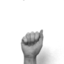
\includegraphics[height=\altura\textheight, keepaspectratio]{ChapterFour/triesch_1.png}}
        \fbox{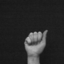
\includegraphics[height=\altura\textheight, keepaspectratio]{ChapterFour/triesch_2.png}}
        \fbox{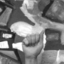
\includegraphics[height=\altura\textheight, keepaspectratio]{ChapterFour/triesch_3.png}} \\\vspace{3px}
        \fbox{
\includegraphics[height=\altura\textheight, keepaspectratio]{ChapterFour/triesch_4.png}}
        \fbox{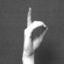
\includegraphics[height=\altura\textheight, keepaspectratio]{ChapterFour/triesch_5.png}}
        \fbox{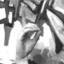
\includegraphics[height=\altura\textheight, keepaspectratio]{ChapterFour/triesch_6.png}} \\\vspace{3px}
        \fbox{
\includegraphics[height=\altura\textheight, keepaspectratio]{ChapterFour/triesch_7.png}}
        \fbox{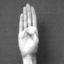
\includegraphics[height=\altura\textheight, keepaspectratio]{ChapterFour/triesch_8.png}}
        \fbox{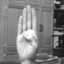
\includegraphics[height=\altura\textheight, keepaspectratio]{ChapterFour/triesch_9.png}}
        \caption{Jochen-Triesch}
        \label{fig:jochen_triesch}
    \end{subfigure}
    \quad
    \begin{subfigure}{0.45\textwidth}
        \centering
        \setlength{\fboxsep}{0pt}
        \fbox{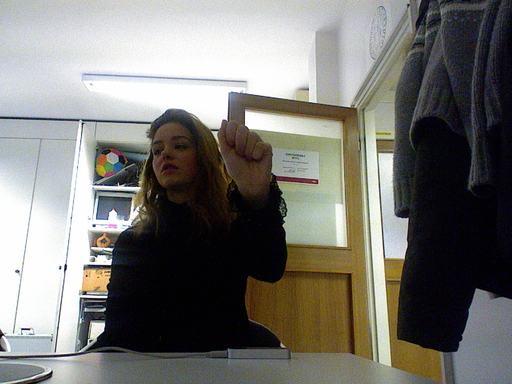
\includegraphics[height=\altura\textheight, keepaspectratio]{ChapterFour/MKLM_1.png}}
        \fbox{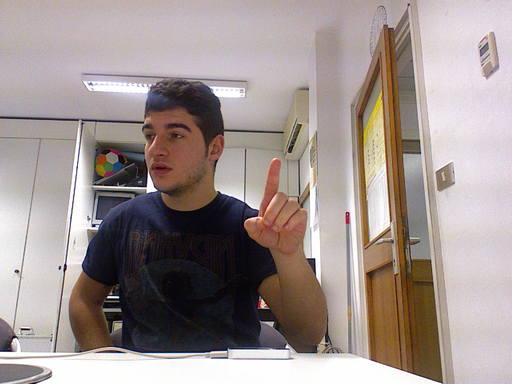
\includegraphics[height=\altura\textheight, keepaspectratio]{ChapterFour/MKLM_2.png}}
        \fbox{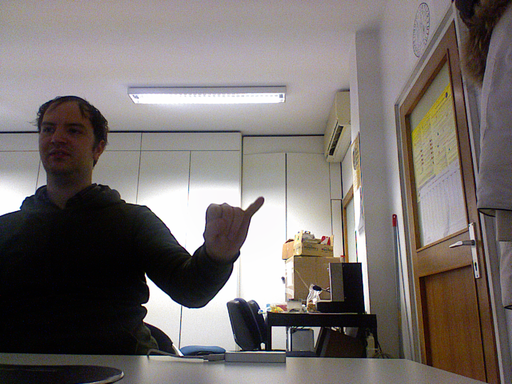
\includegraphics[height=\altura\textheight, keepaspectratio]{ChapterFour/MKLM_3.png}} \\\vspace{3px}
        \fbox{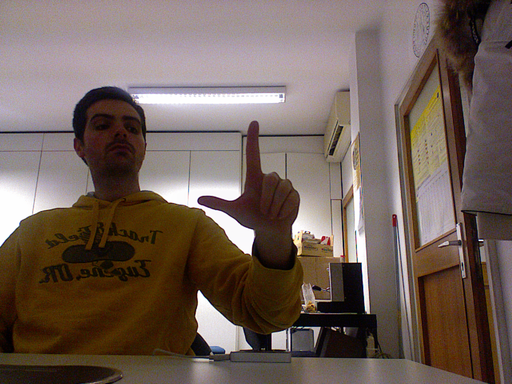
\includegraphics[height=\altura\textheight, keepaspectratio]{ChapterFour/MKLM_4.png}}
        \fbox{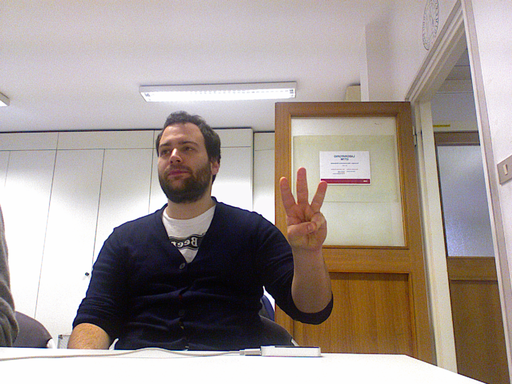
\includegraphics[height=\altura\textheight, keepaspectratio]{ChapterFour/MKLM_6.png}}
        \fbox{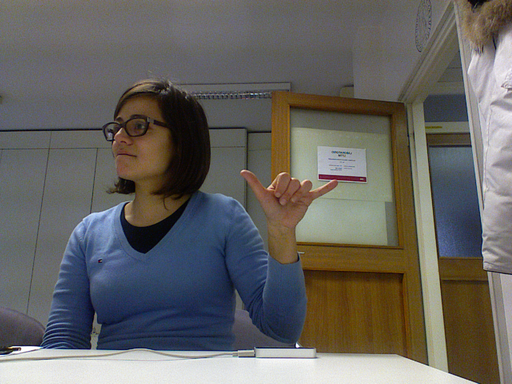
\includegraphics[height=\altura\textheight, keepaspectratio]{ChapterFour/MKLM_7.png}} \\\vspace{3px}
        \fbox{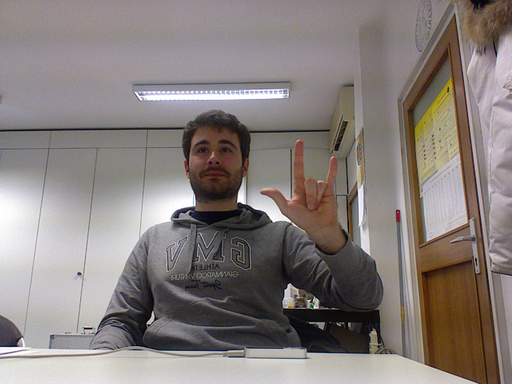
\includegraphics[height=\altura\textheight, keepaspectratio]{ChapterFour/MKLM_8.png}}
        \fbox{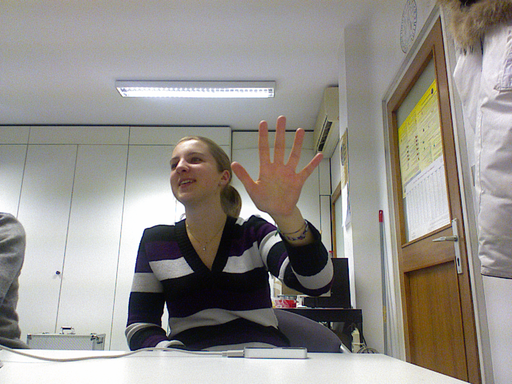
\includegraphics[height=\altura\textheight, keepaspectratio]{ChapterFour/MKLM_9.png}}
        \fbox{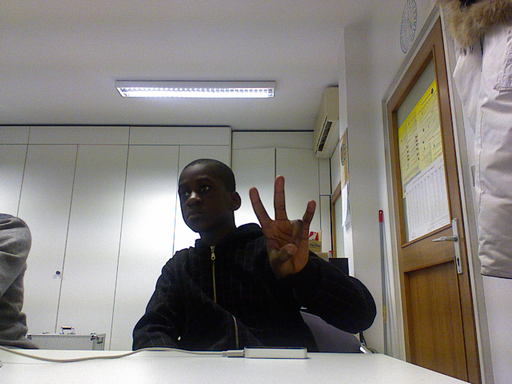
\includegraphics[height=\altura\textheight, keepaspectratio]{ChapterFour/MKLM_10.png}}
        \caption{MKLM}
        \label{fig:mklm}
    \end{subfigure}
    \caption{Illustrative samples of the two datasets used in the experiments.}
    \label{fig:datasets}
\end{figure}

\subsubsection{Baselines}
Throughout this section, the proposed model is compared with state of the art methods for each dataset. Nevertheless, to further attest the robustness of the proposed model, two different baselines are also implemented:
\begin{itemize}
    \item (Baseline 1) A CNN trained from scratch with weight decay regularization. For a fair comparison, the architecture of the baseline CNN corresponds to the architecture of the encoder network followed by the sign-classifier network of the proposed model.
    \item (Baseline 2) A CNN with the baseline 1 topology, but trained with the triplet loss (\citet{Schroff2015}).
\end{itemize}
Here, the triplet loss concept is explored in order to impose signer-independence in the representation space and, hence, build up a more robust baseline. The underlying idea is to minimize the distance between an \textit{anchor} and a \textit{positive} latent representation, $\vz_{y_{i}, s_{i}}$ and $\vz_{y_{p}, s_{p}}$, respectively; while maximizing the distance between the anchor $\vz_{y_{i}, s_{i}}$ and a \textit{negative} representation $\vz_{y_{n}, s_{n}}$. It is important to note that while anchor and positive latent representations have to be from the same sign class, their signer identity may or not change. On the other hand, anchor and negative representations are from different sign classes, whereas their signer identity may also change. In order to train baseline 2 in an end-to-end fashion for sign classification, the overall loss function to be minimized is a trade-off between the triplet loss $L_{\text{triplet}}$, defined below, and the classification loss $L_{\text{sign}}$:
\begin{equation}
L_{\text{triplet}} \triangleq \frac{1}{n}\sum_{i=1}^{n}\Big[||\vz_{y_{i}, s_{i}}-\vz_{y_{p}, s_{p}}||^2_2 - ||\vz_{y_{i}, s_{i}}-\vz_{y_{n}, s_{n}}||^2_2 + \alpha\Big],
\end{equation}
where $y_{p}=y_{i}$ and $y_{n} \neq y_{i}$ and the margin $\alpha$ enforced between \emph{positive} and \emph{negative} pairs was fixed at $\alpha=1$. In addition, following \citet{Schroff2015}, we adopted an \emph{online} triplet generation strategy, by selecting the hardest positive/negative samples within every mini-batch. The overall loss for this model is therefore $L_{\text{sign}} + \rho L_{\text{triplet}}$, where $\rho \geq 0$ is a hyperparameter.

All deep models were implemented in PyTorch and trained with the Adam optimization algorithm using a batch size of 32 samples. For reproducibility purposes, the source code as well as the weights of the trained models are publicly available online\footnote{\url{https://github.com/pmmf/SI-SLR}}. The hyperparameters that are common to all the implemented models (i.e.\ learning rate and $\normltwo$ regularization weight) as well as some hyperparameters that are specific to the proposed model (i.e.\ $\mu_d$ and $\mu_t$) and to the implemented baseline~2 (i.e.\ $\rho$) were optimized by means of a grid search approach and cross-validation on the training set (see \Tableref{tab:hyperparam} for more details). The signer-transfer penalty $L_{\text{transfer}}$ is applied to the last two layers of the encoder network with a relative weight of 1.

\begin{table}[t]
    \centering
        \begin{tabular}{c|c|c}
            Hyperparameters                    & Symbol & Set                \\ \hline
            Leaning rate                                & --      & \{$1\text{e}^{-04}$,$1\text{e}^{-03}$\}             \\
            $\normltwo$-norm coefficient                              & --       & \{$1\text{e}^{-05}$,$1\text{e}^{-04}$\}             \\
            $L_{\text{triplet}}$ weight                 & $\rho$                & \{0.1,0.5,1,5,10\}                  \\
            $L_{\text{adv}}$ weight                 & $\mu_d$                & \{0.1,0.5,0.8,1,3\}                  \\
            $L_{\text{transfer}}$ weight                 & $\mu_t$                & $\{1.5\text{e}^{-04}$,$2\text{e}^{-04}$,$4\text{e}^{-04}$,$1\text{e}^{-03}\}$
        \end{tabular}
    \caption{Hyperparameter sets for the proposed adversarial model and baselines.}
    \label{tab:hyperparam}
\end{table}

\subsubsection{Results and discussion}
Experiments on the Jochen-Triesch and MKLM databases are summarized in \Tableref{tab:adv_signer_inv_results}. We compare our method with other state of the art approaches that have published results on these datasets (\citet{Dahmani2014, Just2006, Kelly2010, Marin2014, Ferreira2018}). The results on the Jochen-Triesch database are presented in terms of average classification accuracy in the overall test set as well as against each specific background type (i.e.\ uniform and complex). For the MKLM database, the table shows the average classification accuracy computed across all test splits, as well as the minimum and maximum accuracy value achieved by each method.

\begin{table}[t]
    \centering
    \resizebox{\linewidth}{!}{
    \begin{tabular}{c|c c c|c c c}
                & \multicolumn{3}{c|}{Jochen Triesch} & \multicolumn{3}{c}{MKLM}\\
                & Uniform  Bg.      & Complex Bg.        & Both  & Avg. $\pm$ std.  & min         & max        \\ \hline
                \citet{Just2006}       & 92.8           & 81.3           & 87.9         & -- & -- & --\\
                \citet{Kelly2010} & 91.8 & -- & -- & -- & -- & --\\
                \citet{Dahmani2014} & 93.1 & -- & -- & -- & -- & --\\
                \citet{Marin2014}  & -- & --  & -- & 89.7 & -- & --\\
                \citet{Ferreira2018} & -- & --  & -- & 93.2 & -- & -- \\
                \hline
                CNN (baseline 1)                            & 97.50           & 74.4           & 89.8   & 89.9 \footnotesize{$\pm 8.8$}            & 73.0                & 98.0\\
                CNN with triplet loss (baseline 2)          & 98.13           & 75.6           & 90.6 & 91.4 \footnotesize{$\pm 3.9$}             & 86.5                & 96.5\\
                Proposed method       &      \textbf{98.8}     & \textbf{91.3}
                & \textbf{96.3} & \textbf{94.8} \footnotesize{$\pm 3.5$}      & \textbf{89.5}
                & \textbf{100.0}
    \end{tabular}}
    \caption{Classification accuracy (\%) of the proposed adversarial method and baselines on Jochen-Triesch and MKLM datasets.}
    \label{tab:adv_signer_inv_results}
\end{table}

The most relevant observation is the superior performance of the proposed model. Specifically, this model exhibits the best overall classification accuracy on both SLR databases, clearly outperforming both implemented baselines and all the previous state of the art models. In Jochen-Triesch, the most challenging data are the images with complex background, where the proposed model surpasses all the remaining by a large margin. In addition, by analyzing the standard deviation as well as the minimum and maximum accuracy values, it is possible to observe that the proposed model is the method with the lowest variability, yielding consistently high accuracy rates across all test splits of the MKLM dataset. These results attest its robustness and capability to better deal with the large inter-signer variability that exists in the manual signing process of sign languages. Interestingly, the obtained results also reveal that the implemented baselines are in fact fairly strong models, both of them outperforming most of the state of the art methods on both datasets.

\Tableref{tab:loss_terms} illustrates the effect of each proposed training scheme by itself. For this purpose, the proposed model was trained either (i) with just the adversarial procedure, without the signer-transfer $L_{\text{transfer}}$ loss, or (ii) with just the $L_{\text{transfer}}$ penalty on the encoder network without adversarial training. The results clearly demonstrate the complementary effect between the two training procedures, as their combination provides the best overall classification accuracy. Interestingly, each training scheme outperforms on its own both baselines and state of the art methods.

\begin{table}[t]
    \centering
    \begin{small}
        \begin{tabular}{c|c c : c }
            & Adversarial ($L_{\text{adv}}$) only  & Signer-transfer ($L_{\text{transfer}}$) only & Both \\ \hline
            Jochen-Triesch                              & 95.2            & 94.4                & \textbf{96.3}        \\
            MKLM            & 94.0            & 94.1                & \textbf{94.8}
        \end{tabular}
    \end{small}
    \caption{\centering The effect of each training procedure in the proposed model. The results in the last column are replicated from \Tableref{tab:adv_signer_inv_results} as they include both training procedures.}
    \label{tab:loss_terms}
\end{table}

\subsubsection{Latent space visualization}
\label{sec:adv_signer_inv_tsne}
To further demonstrate the effectiveness of the proposed model in promoting signer-invariant latent representation spaces, we show in \Figref{fig:adv_signer_inv_tsne} a visual inspection of the latent representations through the t-distributed stochastic neighbor embedding (t-SNE, \citet{Maaten2008}). These plots clearly demonstrate the better capability of the proposed model of imposing signer-independence in the latent representations. The proposed model yields a latent representation space in which representations of different signers and same class are close to each other and well mixed, while it keeps latent representations of different classes far apart. By analyzing the t-SNE plot of baseline 1, it is possible to observe that the latent representations of different signers and the same class tend to be far apart in the latent space. In addition, there is some overlapping between clusters of different classes. Although baseline 2 (CNN with the triplet loss) promoted slightly improvements over the standard baseline CNN, the proposed model achieved by far the best signer-invariance and class separability.

\begin{figure}
    \centering
    \begin{subfigure}[t]{0.32\textwidth}
        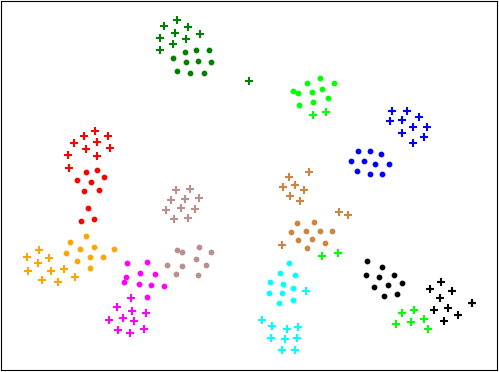
\includegraphics[width=\textwidth]{ChapterFour/tsne_baseline.png}
        \caption{CNN -- baseline 1}
        \label{fig:adv_signer_inv_tsne_a}
    \end{subfigure}
    %\hfill%
    \begin{subfigure}[t]{0.32\textwidth}
        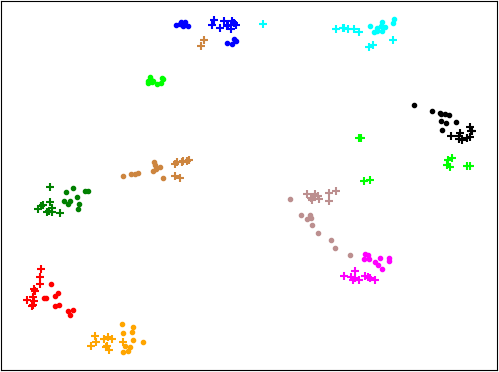
\includegraphics[width=\textwidth]{ChapterFour/tsne_triplet.png}
        \caption{CNN with triplet loss -- baseline 2}
        \label{fig:adv_signer_inv_tsne_b}
    \end{subfigure}
    %\hfill%
    \begin{subfigure}[t]{0.32\textwidth}
        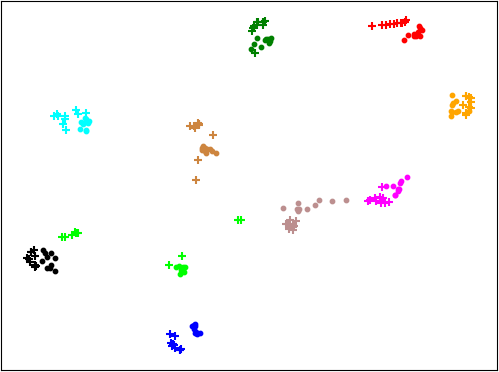
\includegraphics[width=\textwidth]{ChapterFour/tsne_proposed.png}
        \caption{Proposed model}
        \label{fig:adv_signer_inv_tsne_c}
    \end{subfigure}
    \caption{\centering Two-dimensional projection of the latent representation space using the t-distributed stochastic neighbor embedding (t-SNE). Markers $\bullet$ and $\textbf{+}$ represent 2 different test signers, while the different colors denote the 10 sign classes.}
    \label{fig:adv_signer_inv_tsne}
\end{figure}

%-------------------------------------------------------------------------
\subsection{Conclusion}
\label{sec:adv_signer_inv_conclusion}

This paper presents a novel adversarial training objective, based on representation learning and deep neural networks, specifically designed to tackle the signer-independent SLR problem. The underlying idea is to learn signer-invariant latent representations that preserve as much information as possible about the signs, while discarding the signer-specific traits that are irrelevant for sign recognition. For this purpose, we introduce  an adversarial training procedure for simultaneously training an encoder and a sign-classifier over the target sign variables, while preventing the latent representations of the encoder to be predictive of the signer identities. To further discourage the underlying representations of retaining any signer-specific information, we propose an additional training objective that approximates the means of the latent distributions of different signers.
Experimental results demonstrate the effectiveness of the proposed model in several SLR databases.

\section{Adversarial domain generalization for iris presentation attack detection}
\label{sec:adv_iris_attack}
In this section, we show how our adversarial domain generalization model for signer-invariant SLR (presented in \Secref{sec:adv_signer_inv}) can be adapted to a specific biometrics-related application.

\subsection{Introduction}
\label{sec:adv_iris_attack_intro}
Biometric recognition systems are considered reliable enough to be deployed in government and civilian applications. The shift from controlled samples acquisition to a more autonomous one increased the vulnerabilities of these systems. Unfortunately, presentation attack detection (PAD) measures had not grown robustly along with this quick evolution and several weak points can be exploited when performing unsupervised biometric identification as such in mobile biometrics, for example. Successful spoofing attempts have been made public in a matter of days, or even hours, after the release of high-tech devices equipped with biometric recognition. The iris recognition sensor of Samsung S8 was reportedly spoofed by German researchers by simply printing a photo of the authorised user and placing a contact lens in it \cite{cccsamsung2017}. More recently, the quick hack of Samsung Galaxy S10 ultrasonic fingerprint sensor suggests no presentation attack detection measures of any kind. It is fair to conclude that industry does not share the same enthusiasm as academic community on anti-spoofing measures denoted by the good amount of research continuously produced (\citet{raghavendra2015VSIA,czajka2018irisPADreview,Galbally2019,scherhag2019}).

Fortunately, exceptions are starting to show in commercial products, like the recent case of the Apple iPhone ``Face ID'' case\footnote{www.biometricupdate.com/201812/android-devices-facial-recognition-fooled-by-3d-printed-head-but-not-face-id} or the FaceTec ZoOm® technology \cite{facetec102019}. Undoubtedly this change is motivated and supported by initiatives that encourage the development and `open testing' of spoofing coutermeasures such as `The National Voluntary Laboratory Accreditation Program'' (NVLAP) from NIST.\footnote{The NVLAP provides third-party accreditation to testing and calibration laboratories in response to legislative actions or requests from government agencies or private-sector organizations. NVLAP-accredited laboratories are assessed against the management and technical requirements from ISO/IEC 17025:2017.}

Nevertheless, research-wise there are still open problems to address. Here, we focus on the fact that most PAD techniques are based on falsely optimistic evaluation methodologies (\citet{sequeira2016realistic}): traditionally, the classification models are designed and then evaluated using datasets comprising \emph{bona fide} presentations and a specific species of presentation attack instruments (PAI). The case when a PAI in the test set is significantly different from the ones used for training is overlooked. What if such sample has a higher probability to circumvent the system than the ones drawn from the original training dataset? To solve this research question it is necessary to develop robust methods to cope with sophisticated and unseen attacks as our eventual intruders become more capable and successfully develop new spoofing techniques.

The aforementioned problem has been addressed before regarding iris, fingerprint and face (often targeted under the open-set or anomaly detection contexts). However, it still remains a challenging topic. Despite the importance of iris as a biometric trait for recognition purposes, in our view, the study of iris PAD generalization problem to unseen PAI species (PAIS) has not been yet fully studied in literature.

The remainder of this section is organized as follows: i) we start by summarizing the related work on the topic (\Secref{sec:adv_iris_attack_rel_work}); ii) we formalize the problem and emphasize the necessary modifications that had to be done to the model presented in \Secref{sec:adv_signer_inv} to adapt it to this new application (\Secref{sec:adv_iris_attack_method}); iii) we present experimental results that confirm the effectiveness of the model (\Secref{sec:adv_iris_attack_experiments}); iv) we conclude this section with some final remarks (\Secref{sec:adv_iris_attack_conclusion}).

\subsection{Related work}
\label{sec:adv_iris_attack_rel_work}

Recent PAD methods in general, and iris-focused ones in particular, have demonstrated remarkable performances. However, a methodological limitation can be pointed as it is recurrently found that these results are obtained when training and test data comprise the same type of attacks, i.e.\ the same PAIS. This problem has been addressed and proved that the performance rates of these PAD methods typically decrease significantly when the PAIS is new to the system (\citet{marasco2011robustness,bowyer2014cosmetic,sequeira2016realistic}). This performance drop can result from the large inter-PAIS variability. A practical PAD system must operate in a PAIS-independent scenario, which means that the type of PAIS of the test set must not be seen during the training routine of the models. This problem is one of the crucial problems for the development of real-world PAD systems and it has frequently been tackled in literature as an open-set or anomaly detection problem.

The pioneer work that raised the evaluation of PAD methods across different types and unseen PAIS appeared in the fingerprint domain with the work of \citet{marasco2011robustness}. \citet{rattani2015openset} and \citet{sequeira2015fingerprint}, despite using different approaches, both relied on the idea of enforcing the knowledge of the bona fide presentations over the attacks to better deal with unseen PAIS. \citet{bowyer2014cosmetic} studied the evaluation of a binary classification on contact lenses iris spoofing attacks. By using an unseen type on the test set the authors showed that using the same lens types in both the training and testing data can give a very misleading idea of the accuracy of the method.

A step forward was made by combining methodologies designed for print and contact lenses attack (\citet{sequeira2014ildmma}). Eventually, the construction of a new database comprising several types of iris PAIS (\citet{raghavendra2015VSIA}) allowed new evaluation scenarios. \citet{sequeira2016realistic} showed that whenever a new PAIS is presented in the test step, the performance of the classifier drops significantly and that an improvement can be obtained when a one-class classifier is trained only with bona fide presentations.

One-class classification was also used for face by \citet{kittler2017faceanomaly}. With the rise of deep learning (DL) techniques, PAD methods have been proposed applying deep representations for iris, face and fingerprint (\citet{menotti2015deep,pinto2018counteracting}), following the same binary approach. Recent works investigate the robustness of DL fingerprint PAD methods to deal with unseen PAI species (\citet{tolosana2018towards}).

Until recently, most of the proposed approaches either make overly optimistic assumptions about the attacker (binary classification approaches) or only use part of the data (and therefore, of the knowledge) available at training time to design the models (one-class approaches). Therefore, the goal of this work is to present an iris PAD method that uses the information of both bona fide and available attack presentations and is robust to unseen PAI species. This goal will be achieved by enforcing the learning of the task of distinguishing the bona fide from the attack presentations while at the same time ensuring the invariance between the different type of the PAI species.

\subsection{Methodology}
\label{sec:adv_iris_attack_method}
The approach adopted here coincides in most aspects with the one described in \Secref{sec:adv_signer_inv}, so we shall focus on describing the slight differences that exist. Now, the data consists of $\{\mX^{(\text{bf})}_i\}_{i=1}^{n_{\text{bf}}} \cup \{(\mX^{(\text{a})}_i,s_i)\}_{i=1}^{n_{\text{a}}}$, i.e.\ there is one set containing $n_{\text{bf}}$ bona fide examples and another one containing $n_{\text{a}}$ attack examples. Each attack example $\mX^{(\text{a})}_i$ is annotated with the corresponding PAI species label $s_i \in \{1,2,\dots,k\}$.

In this problem, we are solely interested in classifying samples as bona fide or attack, thus $h(\cdot;\vtheta_h)$ (formerly designated as sign-classifier) is now a binary classifier. More importantly, we want to obtain latent representations that are invariant to the PAI species, but the latent representations of bona fide examples should be easily separable from these. Thus, now, only the attack samples are fed through adversarial classifier $d(\cdot;\vtheta_d)$ (formerly designated as signer-classifier) and used for the adversarial training routine. For the same reason, the transfer loss $L_{\text{transfer}}$ approximating first-order statistics only applies to these samples too. \Figref{fig:adv_iris_model} presents the model architecture and hopefully makes the differences between this and our previous model even clearer.

\begin{figure*}[!hbt]
\centering
\tikzset{every picture/.style={line width=0.75pt}} %set default line width to 0.75pt

\scalebox{0.8}{

\tikzset{every picture/.style={line width=0.75pt}} %set default line width to 0.75pt

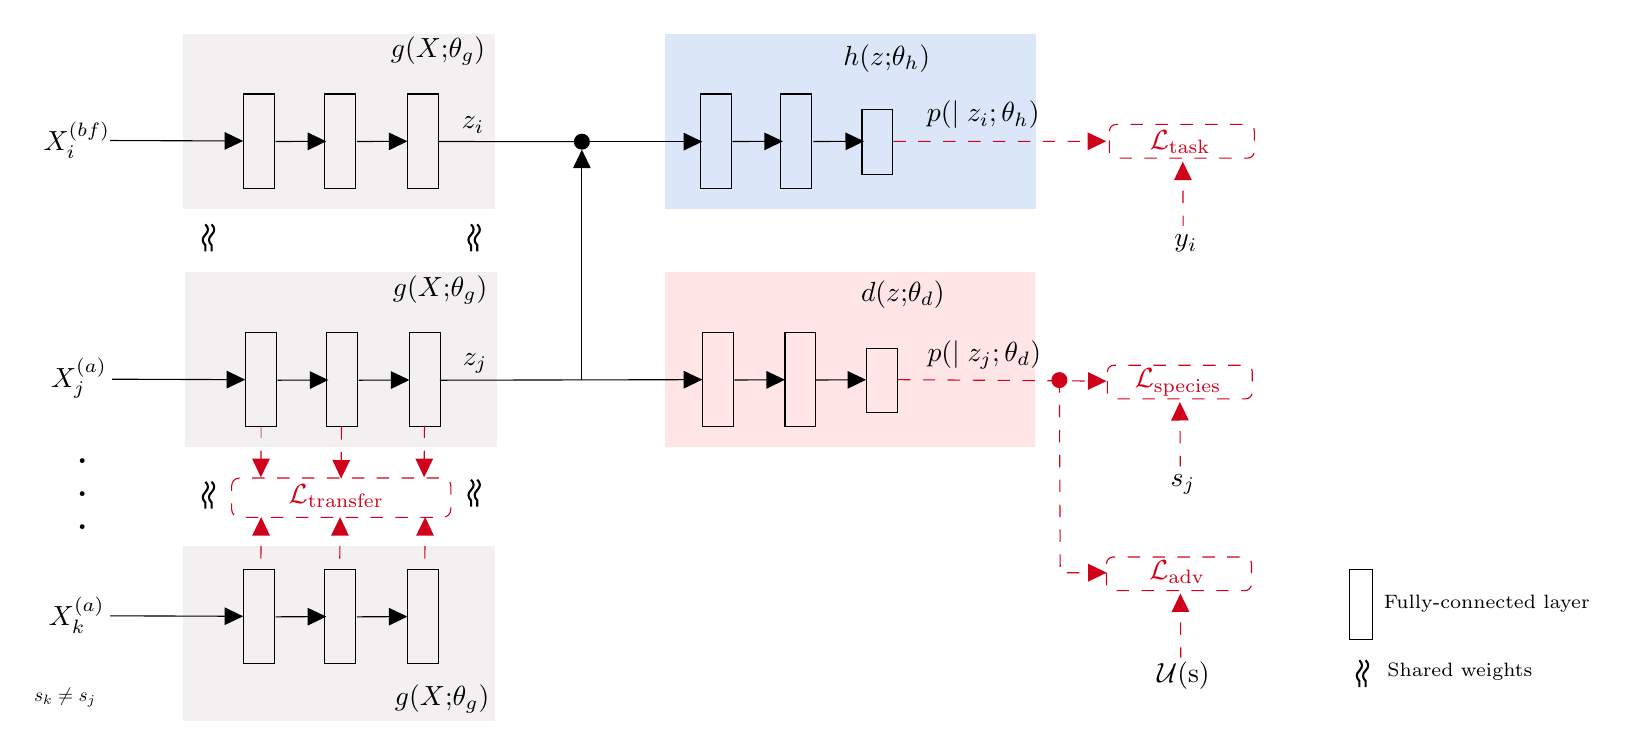
\begin{tikzpicture}[x=0.75pt,y=0.75pt,yscale=-1,xscale=1]
%uncomment if require: \path (0,637); %set diagram left start at 0, and has height of 637

%Shape: Rectangle [id:dp43448545781433445]
\draw  [draw opacity=0][fill={rgb, 255:red, 124; green, 163; blue, 233 }  ,fill opacity=0.27 ][dash pattern={on 4.5pt off 4.5pt}] (342,9) -- (521,9) -- (521,93.23) -- (342,93.23) -- cycle ;
%Shape: Rectangle [id:dp39844785350453726]
\draw   (373.93,38.03) -- (373.93,83.38) -- (359.01,83.38) -- (359.01,38.03) -- cycle ;
%Shape: Rectangle [id:dp5960148926786581]
\draw   (412.75,38.03) -- (412.75,83.38) -- (397.84,83.38) -- (397.84,38.03) -- cycle ;
%Shape: Rectangle [id:dp2968748699957451]
\draw   (451.86,45.72) -- (451.86,76.69) -- (436.94,76.69) -- (436.94,45.72) -- cycle ;
%Straight Lines [id:da38135442637321804]
\draw    (374.47,60.94) -- (396.84,60.84) ;
\draw [shift={(398.84,60.83)}, rotate = 539.75] [fill={rgb, 255:red, 0; green, 0; blue, 0 }  ][line width=0.75]  [draw opacity=0] (8.93,-4.29) -- (0,0) -- (8.93,4.29) -- cycle    ;

%Straight Lines [id:da5103446228646831]
\draw    (413.57,60.94) -- (435.94,60.84) ;
\draw [shift={(437.94,60.83)}, rotate = 539.75] [fill={rgb, 255:red, 0; green, 0; blue, 0 }  ][line width=0.75]  [draw opacity=0] (8.93,-4.29) -- (0,0) -- (8.93,4.29) -- cycle    ;

%Shape: Rectangle [id:dp21504155648063916]
\draw  [draw opacity=0][fill={rgb, 255:red, 255; green, 199; blue, 199 }  ,fill opacity=0.46 ][dash pattern={on 4.5pt off 4.5pt}] (342.06,123.9) -- (520.25,123.9) -- (520.25,208.13) -- (342.06,208.13) -- cycle ;
%Shape: Rectangle [id:dp5629086137047858]
\draw   (374.93,152.92) -- (374.93,198.28) -- (360.01,198.28) -- (360.01,152.92) -- cycle ;
%Shape: Rectangle [id:dp11383387176162141]
\draw   (414.75,152.92) -- (414.75,198.28) -- (399.84,198.28) -- (399.84,152.92) -- cycle ;
%Shape: Rectangle [id:dp8834314863600405]
\draw   (453.86,160.61) -- (453.86,191.59) -- (438.94,191.59) -- (438.94,160.61) -- cycle ;
%Straight Lines [id:da7960584409422926]
\draw    (375.47,175.84) -- (397.84,175.74) ;
\draw [shift={(399.84,175.73)}, rotate = 539.75] [fill={rgb, 255:red, 0; green, 0; blue, 0 }  ][line width=0.75]  [draw opacity=0] (8.93,-4.29) -- (0,0) -- (8.93,4.29) -- cycle    ;

%Straight Lines [id:da26603179330471005]
\draw    (414.57,175.84) -- (436.94,175.74) ;
\draw [shift={(438.94,175.73)}, rotate = 539.75] [fill={rgb, 255:red, 0; green, 0; blue, 0 }  ][line width=0.75]  [draw opacity=0] (8.93,-4.29) -- (0,0) -- (8.93,4.29) -- cycle    ;

%Straight Lines [id:da43094599217232044]
\draw [color={rgb, 255:red, 208; green, 2; blue, 27 }  ,draw opacity=1 ] [dash pattern={on 4.5pt off 4.5pt}]  (452.06,60.88) -- (552.61,60.84) ;
\draw [shift={(554.61,60.83)}, rotate = 539.98] [fill={rgb, 255:red, 208; green, 2; blue, 27 }  ,fill opacity=1 ][line width=0.75]  [draw opacity=0] (8.93,-4.29) -- (0,0) -- (8.93,4.29) -- cycle    ;

%Rounded Rect [id:dp20102262667247417]
\draw  [color={rgb, 255:red, 208; green, 2; blue, 27 }  ,draw opacity=1 ][dash pattern={on 4.5pt off 4.5pt}] (555.16,171.96) .. controls (555.16,170.16) and (556.62,168.71) .. (558.41,168.71) -- (621.75,168.71) .. controls (623.55,168.71) and (625,170.16) .. (625,171.96) -- (625,181.69) .. controls (625,183.48) and (623.55,184.94) .. (621.75,184.94) -- (558.41,184.94) .. controls (556.62,184.94) and (555.16,183.48) .. (555.16,181.69) -- cycle ;
%Straight Lines [id:da7107772326187543]
\draw [color={rgb, 255:red, 208; green, 2; blue, 27 }  ,draw opacity=1 ] [dash pattern={on 4.5pt off 4.5pt}]  (454.25,175.67) -- (552.78,176.37) ;
\draw [shift={(554.78,176.38)}, rotate = 180.41] [fill={rgb, 255:red, 208; green, 2; blue, 27 }  ,fill opacity=1 ][line width=0.75]  [draw opacity=0] (8.93,-4.29) -- (0,0) -- (8.93,4.29) -- cycle    ;

%Straight Lines [id:da7856916848123423]
\draw [color={rgb, 255:red, 208; green, 2; blue, 27 }  ,draw opacity=1 ] [dash pattern={on 4.5pt off 4.5pt}]  (147.5,197.88) -- (147.35,220.67) ;
\draw [shift={(147.33,222.67)}, rotate = 270.39] [fill={rgb, 255:red, 208; green, 2; blue, 27 }  ,fill opacity=1 ][line width=0.75]  [draw opacity=0] (8.93,-4.29) -- (0,0) -- (8.93,4.29) -- cycle    ;

%Straight Lines [id:da36002582240035363]
\draw [color={rgb, 255:red, 0; green, 0; blue, 0 }  ,draw opacity=1 ][line width=0.75]    (251.6,223.85) .. controls (253.27,225.52) and (253.27,227.18) .. (251.6,228.85) .. controls (249.93,230.52) and (249.93,232.18) .. (251.6,233.85) -- (251.6,236.85) -- (251.6,236.85)(248.6,223.85) .. controls (250.27,225.52) and (250.27,227.18) .. (248.6,228.85) .. controls (246.93,230.52) and (246.93,232.18) .. (248.6,233.85) -- (248.6,236.85) -- (248.6,236.85) ;


%Rounded Rect [id:dp28118263286951617]
\draw  [color={rgb, 255:red, 208; green, 2; blue, 27 }  ,draw opacity=1 ][dash pattern={on 4.5pt off 4.5pt}] (556.16,55.96) .. controls (556.16,54.16) and (557.62,52.71) .. (559.41,52.71) -- (622.75,52.71) .. controls (624.55,52.71) and (626,54.16) .. (626,55.96) -- (626,65.69) .. controls (626,67.48) and (624.55,68.94) .. (622.75,68.94) -- (559.41,68.94) .. controls (557.62,68.94) and (556.16,67.48) .. (556.16,65.69) -- cycle ;
%Straight Lines [id:da5356763271282314]
\draw [color={rgb, 255:red, 208; green, 2; blue, 27 }  ,draw opacity=1 ] [dash pattern={on 4.5pt off 4.5pt}]  (591.52,72.62) -- (591.71,101.6) ;

\draw [shift={(591.51,70.62)}, rotate = 89.63] [fill={rgb, 255:red, 208; green, 2; blue, 27 }  ,fill opacity=1 ][line width=0.75]  [draw opacity=0] (8.93,-4.29) -- (0,0) -- (8.93,4.29) -- cycle    ;
%Straight Lines [id:da9155638065763507]
\draw [color={rgb, 255:red, 208; green, 2; blue, 27 }  ,draw opacity=1 ] [dash pattern={on 4.5pt off 4.5pt}]  (590.12,188.42) -- (590.31,217.4) ;

\draw [shift={(590.11,186.42)}, rotate = 89.63] [fill={rgb, 255:red, 208; green, 2; blue, 27 }  ,fill opacity=1 ][line width=0.75]  [draw opacity=0] (8.93,-4.29) -- (0,0) -- (8.93,4.29) -- cycle    ;
%Straight Lines [id:da7191094178180941]
\draw [color={rgb, 255:red, 0; green, 0; blue, 0 }  ,draw opacity=1 ][line width=0.75]    (123.6,100.85) .. controls (125.27,102.52) and (125.27,104.18) .. (123.6,105.85) .. controls (121.93,107.52) and (121.93,109.18) .. (123.6,110.85) -- (123.6,113.85) -- (123.6,113.85)(120.6,100.85) .. controls (122.27,102.52) and (122.27,104.18) .. (120.6,105.85) .. controls (118.93,107.52) and (118.93,109.18) .. (120.6,110.85) -- (120.6,113.85) -- (120.6,113.85) ;


%Rounded Rect [id:dp5531536926433998]
\draw  [color={rgb, 255:red, 208; green, 2; blue, 27 }  ,draw opacity=1 ][dash pattern={on 4.5pt off 4.5pt}] (133.28,226.86) .. controls (133.28,224.77) and (134.98,223.07) .. (137.07,223.07) -- (235.08,223.07) .. controls (237.17,223.07) and (238.86,224.77) .. (238.86,226.86) -- (238.86,238.21) .. controls (238.86,240.31) and (237.17,242) .. (235.08,242) -- (137.07,242) .. controls (134.98,242) and (133.28,240.31) .. (133.28,238.21) -- cycle ;
%Straight Lines [id:da6744189660599909]
\draw [color={rgb, 255:red, 208; green, 2; blue, 27 }  ,draw opacity=1 ] [dash pattern={on 4.5pt off 4.5pt}]  (532.07,175.88) -- (532.47,268.68) -- (552.87,268.68) ;
\draw [shift={(554.87,268.68)}, rotate = 180] [fill={rgb, 255:red, 208; green, 2; blue, 27 }  ,fill opacity=1 ][line width=0.75]  [draw opacity=0] (8.93,-4.29) -- (0,0) -- (8.93,4.29) -- cycle    ;
\draw [shift={(532.07,175.88)}, rotate = 89.75] [color={rgb, 255:red, 208; green, 2; blue, 27 }  ,draw opacity=1 ][fill={rgb, 255:red, 208; green, 2; blue, 27 }  ,fill opacity=1 ][line width=0.75]      (0, 0) circle [x radius= 3.35, y radius= 3.35]   ;
%Rounded Rect [id:dp27586876312894315]
\draw  [color={rgb, 255:red, 208; green, 2; blue, 27 }  ,draw opacity=1 ][dash pattern={on 4.5pt off 4.5pt}] (554.76,264.36) .. controls (554.76,262.56) and (556.22,261.11) .. (558.01,261.11) -- (621.35,261.11) .. controls (623.15,261.11) and (624.6,262.56) .. (624.6,264.36) -- (624.6,274.09) .. controls (624.6,275.88) and (623.15,277.34) .. (621.35,277.34) -- (558.01,277.34) .. controls (556.22,277.34) and (554.76,275.88) .. (554.76,274.09) -- cycle ;
%Straight Lines [id:da05722319267703546]
\draw [color={rgb, 255:red, 208; green, 2; blue, 27 }  ,draw opacity=1 ] [dash pattern={on 4.5pt off 4.5pt}]  (590.37,280.67) -- (590.56,309.65) ;

\draw [shift={(590.36,278.67)}, rotate = 89.63] [fill={rgb, 255:red, 208; green, 2; blue, 27 }  ,fill opacity=1 ][line width=0.75]  [draw opacity=0] (8.93,-4.29) -- (0,0) -- (8.93,4.29) -- cycle    ;
%Shape: Rectangle [id:dp5258454923666749]
\draw   (683,267) -- (683,301) -- (671.91,301) -- (671.91,267) -- cycle ;
%Shape: Rectangle [id:dp18819058590818738]
\draw  [draw opacity=0][fill={rgb, 255:red, 226; green, 223; blue, 223 }  ,fill opacity=0.46 ][dash pattern={on 4.5pt off 4.5pt}] (110,9) -- (260.3,9) -- (260.3,93.23) -- (110,93.23) -- cycle ;
%Shape: Rectangle [id:dp12041639376004776]
\draw   (153.93,38.03) -- (153.93,83.38) -- (139.01,83.38) -- (139.01,38.03) -- cycle ;
%Shape: Rectangle [id:dp8185093400372612]
\draw   (192.75,38.03) -- (192.75,83.38) -- (177.84,83.38) -- (177.84,38.03) -- cycle ;
%Straight Lines [id:da46781806052292585]
\draw    (154.47,60.94) -- (176.84,60.84) ;
\draw [shift={(178.84,60.83)}, rotate = 539.75] [fill={rgb, 255:red, 0; green, 0; blue, 0 }  ][line width=0.75]  [draw opacity=0] (8.93,-4.29) -- (0,0) -- (8.93,4.29) -- cycle    ;

%Straight Lines [id:da8380691205174686]
\draw    (193.57,60.94) -- (215.94,60.84) ;
\draw [shift={(217.94,60.83)}, rotate = 539.75] [fill={rgb, 255:red, 0; green, 0; blue, 0 }  ][line width=0.75]  [draw opacity=0] (8.93,-4.29) -- (0,0) -- (8.93,4.29) -- cycle    ;

%Shape: Rectangle [id:dp7823549329526485]
\draw   (232.75,38.03) -- (232.75,83.38) -- (217.84,83.38) -- (217.84,38.03) -- cycle ;
%Straight Lines [id:da8112293131002832]
\draw    (232.57,60.94) -- (302,61) ;
\draw [shift={(302,61)}, rotate = 0.05] [color={rgb, 255:red, 0; green, 0; blue, 0 }  ][fill={rgb, 255:red, 0; green, 0; blue, 0 }  ][line width=0.75]      (0, 0) circle [x radius= 3.35, y radius= 3.35]   ;

%Straight Lines [id:da3383332186453154]
\draw    (74.69,60.46) -- (136.8,60.67) ;
\draw [shift={(138.8,60.68)}, rotate = 180.19] [fill={rgb, 255:red, 0; green, 0; blue, 0 }  ][line width=0.75]  [draw opacity=0] (8.93,-4.29) -- (0,0) -- (8.93,4.29) -- cycle    ;

%Shape: Rectangle [id:dp4074002721672936]
\draw  [draw opacity=0][fill={rgb, 255:red, 226; green, 223; blue, 223 }  ,fill opacity=0.46 ][dash pattern={on 4.5pt off 4.5pt}] (111,124) -- (261.3,124) -- (261.3,208.23) -- (111,208.23) -- cycle ;
%Shape: Rectangle [id:dp5490194067870466]
\draw   (154.93,153.03) -- (154.93,198.38) -- (140.01,198.38) -- (140.01,153.03) -- cycle ;
%Shape: Rectangle [id:dp5328143148819742]
\draw   (193.75,153.03) -- (193.75,198.38) -- (178.84,198.38) -- (178.84,153.03) -- cycle ;
%Straight Lines [id:da5553578784490631]
\draw    (155.47,175.94) -- (177.84,175.84) ;
\draw [shift={(179.84,175.83)}, rotate = 539.75] [fill={rgb, 255:red, 0; green, 0; blue, 0 }  ][line width=0.75]  [draw opacity=0] (8.93,-4.29) -- (0,0) -- (8.93,4.29) -- cycle    ;

%Straight Lines [id:da013990047318108267]
\draw    (194.57,175.94) -- (216.94,175.84) ;
\draw [shift={(218.94,175.83)}, rotate = 539.75] [fill={rgb, 255:red, 0; green, 0; blue, 0 }  ][line width=0.75]  [draw opacity=0] (8.93,-4.29) -- (0,0) -- (8.93,4.29) -- cycle    ;

%Shape: Rectangle [id:dp8533827475188887]
\draw   (233.75,153.03) -- (233.75,198.38) -- (218.84,198.38) -- (218.84,153.03) -- cycle ;
%Straight Lines [id:da9882205897592524]
\draw    (233.57,175.94) -- (358,175.67) ;
\draw [shift={(360,175.67)}, rotate = 539.87] [fill={rgb, 255:red, 0; green, 0; blue, 0 }  ][line width=0.75]  [draw opacity=0] (8.93,-4.29) -- (0,0) -- (8.93,4.29) -- cycle    ;

%Straight Lines [id:da787593595255915]
\draw    (75.69,175.46) -- (137.8,175.67) ;
\draw [shift={(139.8,175.68)}, rotate = 180.19] [fill={rgb, 255:red, 0; green, 0; blue, 0 }  ][line width=0.75]  [draw opacity=0] (8.93,-4.29) -- (0,0) -- (8.93,4.29) -- cycle    ;

%Shape: Rectangle [id:dp9669269547137105]
\draw  [draw opacity=0][fill={rgb, 255:red, 226; green, 223; blue, 223 }  ,fill opacity=0.46 ][dash pattern={on 4.5pt off 4.5pt}] (110,256) -- (260.3,256) -- (260.3,340.23) -- (110,340.23) -- cycle ;
%Shape: Rectangle [id:dp042461560729392334]
\draw   (153.93,267.03) -- (153.93,312.38) -- (139.01,312.38) -- (139.01,267.03) -- cycle ;
%Shape: Rectangle [id:dp05976855107797907]
\draw   (192.75,267.03) -- (192.75,312.38) -- (177.84,312.38) -- (177.84,267.03) -- cycle ;
%Straight Lines [id:da15536321808735676]
\draw    (154.47,289.94) -- (176.84,289.84) ;
\draw [shift={(178.84,289.83)}, rotate = 539.75] [fill={rgb, 255:red, 0; green, 0; blue, 0 }  ][line width=0.75]  [draw opacity=0] (8.93,-4.29) -- (0,0) -- (8.93,4.29) -- cycle    ;

%Straight Lines [id:da390775000910931]
\draw    (193.57,289.94) -- (215.94,289.84) ;
\draw [shift={(217.94,289.83)}, rotate = 539.75] [fill={rgb, 255:red, 0; green, 0; blue, 0 }  ][line width=0.75]  [draw opacity=0] (8.93,-4.29) -- (0,0) -- (8.93,4.29) -- cycle    ;

%Shape: Rectangle [id:dp6405433268349929]
\draw   (232.75,267.03) -- (232.75,312.38) -- (217.84,312.38) -- (217.84,267.03) -- cycle ;
%Straight Lines [id:da12900931641427915]
\draw    (74.69,289.46) -- (136.8,289.67) ;
\draw [shift={(138.8,289.68)}, rotate = 180.19] [fill={rgb, 255:red, 0; green, 0; blue, 0 }  ][line width=0.75]  [draw opacity=0] (8.93,-4.29) -- (0,0) -- (8.93,4.29) -- cycle    ;

%Straight Lines [id:da6895522275561663]
\draw [color={rgb, 255:red, 208; green, 2; blue, 27 }  ,draw opacity=1 ] [dash pattern={on 4.5pt off 4.5pt}]  (186.17,198.54) -- (186.01,221.33) ;
\draw [shift={(186,223.33)}, rotate = 270.39] [fill={rgb, 255:red, 208; green, 2; blue, 27 }  ,fill opacity=1 ][line width=0.75]  [draw opacity=0] (8.93,-4.29) -- (0,0) -- (8.93,4.29) -- cycle    ;

%Straight Lines [id:da7826731128924016]
\draw [color={rgb, 255:red, 208; green, 2; blue, 27 }  ,draw opacity=1 ] [dash pattern={on 4.5pt off 4.5pt}]  (226.17,197.88) -- (226.01,220.67) ;
\draw [shift={(226,222.67)}, rotate = 270.39] [fill={rgb, 255:red, 208; green, 2; blue, 27 }  ,fill opacity=1 ][line width=0.75]  [draw opacity=0] (8.93,-4.29) -- (0,0) -- (8.93,4.29) -- cycle    ;

%Straight Lines [id:da04218018142765656]
\draw [color={rgb, 255:red, 208; green, 2; blue, 27 }  ,draw opacity=1 ] [dash pattern={on 4.5pt off 4.5pt}]  (147.49,243.87) -- (147.33,266.67) ;

\draw [shift={(147.5,241.88)}, rotate = 90.39] [fill={rgb, 255:red, 208; green, 2; blue, 27 }  ,fill opacity=1 ][line width=0.75]  [draw opacity=0] (8.93,-4.29) -- (0,0) -- (8.93,4.29) -- cycle    ;
%Straight Lines [id:da31456133747342974]
\draw [color={rgb, 255:red, 208; green, 2; blue, 27 }  ,draw opacity=1 ] [dash pattern={on 4.5pt off 4.5pt}]  (185.49,243.87) -- (185.33,266.67) ;

\draw [shift={(185.5,241.88)}, rotate = 90.39] [fill={rgb, 255:red, 208; green, 2; blue, 27 }  ,fill opacity=1 ][line width=0.75]  [draw opacity=0] (8.93,-4.29) -- (0,0) -- (8.93,4.29) -- cycle    ;
%Straight Lines [id:da5649357265644332]
\draw [color={rgb, 255:red, 208; green, 2; blue, 27 }  ,draw opacity=1 ] [dash pattern={on 4.5pt off 4.5pt}]  (226.49,243.87) -- (226.33,266.67) ;

\draw [shift={(226.5,241.88)}, rotate = 90.39] [fill={rgb, 255:red, 208; green, 2; blue, 27 }  ,fill opacity=1 ][line width=0.75]  [draw opacity=0] (8.93,-4.29) -- (0,0) -- (8.93,4.29) -- cycle    ;
%Straight Lines [id:da21749981772402482]
\draw    (302,176) -- (302,66.83) ;
\draw [shift={(302,64.83)}, rotate = 450] [fill={rgb, 255:red, 0; green, 0; blue, 0 }  ][line width=0.75]  [draw opacity=0] (8.93,-4.29) -- (0,0) -- (8.93,4.29) -- cycle    ;

%Straight Lines [id:da8956250937163148]
\draw [color={rgb, 255:red, 0; green, 0; blue, 0 }  ,draw opacity=1 ][line width=0.75]    (123.6,224.85) .. controls (125.27,226.52) and (125.27,228.18) .. (123.6,229.85) .. controls (121.93,231.52) and (121.93,233.18) .. (123.6,234.85) -- (123.6,237.85) -- (123.6,237.85)(120.6,224.85) .. controls (122.27,226.52) and (122.27,228.18) .. (120.6,229.85) .. controls (118.93,231.52) and (118.93,233.18) .. (120.6,234.85) -- (120.6,237.85) -- (120.6,237.85) ;


%Straight Lines [id:da9131455128555723]
\draw [color={rgb, 255:red, 0; green, 0; blue, 0 }  ,draw opacity=1 ][line width=0.75]    (251.6,100.85) .. controls (253.27,102.52) and (253.27,104.18) .. (251.6,105.85) .. controls (249.93,107.52) and (249.93,109.18) .. (251.6,110.85) -- (251.6,113.85) -- (251.6,113.85)(248.6,100.85) .. controls (250.27,102.52) and (250.27,104.18) .. (248.6,105.85) .. controls (246.93,107.52) and (246.93,109.18) .. (248.6,110.85) -- (248.6,113.85) -- (248.6,113.85) ;


%Straight Lines [id:da34712918534938386]
\draw [color={rgb, 255:red, 0; green, 0; blue, 0 }  ,draw opacity=1 ][line width=0.75]    (679.6,310.85) .. controls (681.27,312.52) and (681.27,314.18) .. (679.6,315.85) .. controls (677.93,317.52) and (677.93,319.18) .. (679.6,320.85) -- (679.6,323.85) -- (679.6,323.85)(676.6,310.85) .. controls (678.27,312.52) and (678.27,314.18) .. (676.6,315.85) .. controls (674.93,317.52) and (674.93,319.18) .. (676.6,320.85) -- (676.6,323.85) -- (676.6,323.85) ;


%Straight Lines [id:da3483077683758504]
\draw    (302,61) -- (358,61) ;
\draw [shift={(360,61)}, rotate = 180] [fill={rgb, 255:red, 0; green, 0; blue, 0 }  ][line width=0.75]  [draw opacity=0] (8.93,-4.29) -- (0,0) -- (8.93,4.29) -- cycle    ;


% Text Node
\draw (58.68,60.11) node   {$\boldsymbol{X}^{(\text{bf})}_{i}$};
% Text Node
\draw (61.35,230.89) node  [align=left] {\textbf{{\large .}}\\\textbf{{\large .}}\\\textbf{{\large .}}};
% Text Node
\draw (448.89,20.95) node   {$h(\boldsymbol{z}\mathrm{;}\boldsymbol{\theta} _{h})$};
% Text Node
\draw (456.63,134.64) node   {$d(\boldsymbol{z}\mathrm{;}\boldsymbol{\theta} _{d})$};
% Text Node
\draw (589.25,177.03) node   {${\textstyle \mathcal{\textcolor[rgb]{0.82,0.01,0.11}{L}}\textcolor[rgb]{0.82,0.01,0.11}{_{\mathrm{species}}}}$};
% Text Node
\draw (495.39,48.2) node   {$p( \ry \mid \boldsymbol{z}_{i} ;\boldsymbol{\theta} _{h})$};
% Text Node
\draw (249.56,53.01) node   {$\boldsymbol{z}_{i}$};
% Text Node
\draw (183.66,231.92) node   {${\textstyle \mathcal{\textcolor[rgb]{0.82,0.01,0.11}{L}}\textcolor[rgb]{0.82,0.01,0.11}{_{\mathrm{transfer}}}}$};
% Text Node
\draw (590.25,61.03) node   {${\textstyle \mathcal{\textcolor[rgb]{0.82,0.01,0.11}{L}}\textcolor[rgb]{0.82,0.01,0.11}{_{\mathrm{task}}}}$};
% Text Node
\draw (593,110.17) node   {$y_{i}$};
% Text Node
\draw (591.6,225.97) node   {$s_{j}$};
% Text Node
\draw (588.85,268.43) node   {${\textstyle \mathcal{\textcolor[rgb]{0.82,0.01,0.11}{L}}\textcolor[rgb]{0.82,0.01,0.11}{_{\mathrm{adv}}}}$};
% Text Node
\draw (591.85,318.22) node   {$\mathcal{U}(\mathrm{s})$};
% Text Node
\draw (738,283.5) node  [align=left] {{\scriptsize Fully-connected layer}};
% Text Node
\draw (52.96,329) node [scale=0.7]  {$\mathnormal{s_{k} \neq s_{j}}$};
% Text Node
\draw (495.89,163.7) node   {$p( \rs \mid \boldsymbol{z}_{j} ;\boldsymbol{\theta} _{d})$};
% Text Node
\draw (232.7,17.44) node   {$g(\boldsymbol{X}\mathrm{;}\boldsymbol{\theta} _{g})$};
% Text Node
\draw (59.68,175.11) node   {$\boldsymbol{X}^{(\text{a})}_{j}$};
% Text Node
\draw (250.56,168.01) node   {$\boldsymbol{z}_{j}$};
% Text Node
\draw (233.7,132.44) node   {$g(\boldsymbol{X}\mathrm{;}\boldsymbol{\theta} _{g})$};
% Text Node
\draw (58.68,289.11) node   {$\boldsymbol{X}^{(\text{a})}_{k}$};
% Text Node
\draw (234.7,329.44) node   {$g(\boldsymbol{X}\mathrm{;}\boldsymbol{\theta} _{g})$};
% Text Node
\draw (725,316.5) node  [align=left] {{\scriptsize Shared weights}};
\end{tikzpicture}
}
\caption{Block diagram of the proposed species-invariant neural network.}
\label{fig:adv_iris_model}
\end{figure*}


\subsection{Experiments}
\label{sec:adv_iris_attack_experiments}
We use the Visible Spectrum Iris Artefact (VSIA) database (\citet{raghavendra2015VSIA}) in our experiments. This dataset comprises five different presentations combining print and electronic screen attacks: i) Print Attack (PA); ii) iPad Electronic Screen Attack (ESA); iii) Samsung Galaxy Tab ESA; iv) combined PA \& ESA using iPad; and v) combined PA \& ESA using Samsung Pad. The methods are evaluated by leaving out one PAI species for testing. The development set is therefore divided into one species for validation and the remaining for training. Also the same set of samples are used for testing across the different experiments to allow precise comparison of the results. Following \citet{sequeira2016realistic}, weighted local binary pattern features (wLBP, \citet{zhang2010contact}) were extracted in a preprocessing step and fed as input to the network, which in this case consists of an MLP.

Our model was compared to a baseline consisting of the same classifier without the PAI species classifier and adversarial training and to an SVM operating on top of the same wLBP features (\citet{sequeira2016realistic}). Results are in \Tableref{tab:pad_accuracy}. Comparing the accuracy for each attack, it can be observed that uniquely replacing the SVM with an MLP does not result in an improvement. This can be explained by the fact that the dataset has a very limited size and therefore the MLP method tends to overfit due to the lack of training samples. It was not for no reason that SVMs ruled for a long time in the pattern recognition domain. However, the proposed adversarial approach outperformed the SVM for most attacks and on average as well.

For further results and details about the experiments, please see \citet{AdvInvAttack}.

\begin{table}[t]
    \centering
    \begin{small}
        \begin{tabular}{c|c c c c c:c}
            & Attack i)
            & Attack ii)
            & Attack iii)
            & Attack iv)
            & Attack v)
            & Avg. \\ \hline

            wLBP+SVM~\cite{sequeira2016realistic}
            &78.9     &90.4     &\bf 98.1 &\bf 95.7 & 97.1     & 92.0 \\
            Baseline wLBP+MLP
            &78.0     &\bf 93.0  &94.5    &90.0   &95.5     &90.2 \\
            Proposed wLBP+$\text{MLP}_\text{adv}$
            &\bf82.0  &\bf 93.0  &98.0   &94.5   &\bf 97.5  &\bf 93.0
        \end{tabular}
    \end{small}
    \caption{Presentation attack detection accuracy (\%) in the VSIA dataset.}
    \label{tab:pad_accuracy}
\end{table}

\subsection{Conclusion}
\label{sec:adv_iris_attack_conclusion}
This work proposed a method to improve the robustness and generalization capacity of an iris PAD method to new attacks. The goal of the proposed model is to learn latent representations invariant to the PAI species that preserve relevant information about the PAD properties while discarding the `PAI-species'-specific aspects that may hamper the PAD classification task. The proposed regularization strategies made the PAD method `PAI-species'-independent and robust to new test PAIS.
The experiments were based in comparing a baseline MLP and an MLP trained with adversarial strategies using as input highly discriminative features (wLBP) extracted from the images. When comparing the baseline MLP to an SVM classifier the results are quite similar or even worse. This can be explained simply by the fact that the dataset has a very limited size and the MLP method will overfit.
However, applying the adversarial regularization strategy significantly improved the PAD robustness of the method. The obtained results clearly suggest that the application of deep learning techniques with additional strategies will provide breakthroughs in this challenge.

\section{DeSIRe: Deep Signer-Invariant Representations for Sign Language Recognition}
\label{sec:desire}

\subsection{Introduction}
In \Secref{sec:adv_signer_inv}, we introduced a method for domain generalization which uses adversarial neural networks to align the marginal distributions of multiple source domains. The method showed promising results for both visual (\Secref{sec:adv_signer_inv}) and non-visual data (\Secref{sec:adv_iris_attack}). Here, we again focus our attention on vision problems and, specifically, on solving the problem of signer-independent SLR.

To specifically tackle the signer-independent SLR problem, we now present DeSIRe, a novel deep neural network that aims to learn \underline{De}ep \underline{S}igner-\underline{I}nvariant \underline{Re}presentations. The underlying idea is to explicitly enforce the model to automatically learn highly discriminative signer-invariant feature representations from the data by aligning and regularizing conditional distributions in a latent space. To accomplish this goal, the DeSIRe model consists of two main modules or components, namely a conditional variational autoencoder (CVAE) and a classifier. Specifically, the main task of the CVAE is to explicitly impose signer independence on the learned latent representations. This is achieved by encouraging the CVAE to learn latent representations whose conditional posterior distribution (given the image and the corresponding sign class label) is independent of the signer identity. Accordingly, the learned latent representations will preserve as much information as possible about the class (sign) and discard the irrelevant parts that are signer-specific. In addition, the CVAE acts as a teacher model for the classifier since the distribution over latent representations is used to regularize the hidden representations of the classifier. These hidden representations are then fed into a multilayer perceptron (MLP) for sign classification. The result is a signer-independent model robust to new test signers.

The remainder of this section is organized as follows: i) the proposed signer-independent deep neural network along with the proposed loss function and regularization schemes are fully described in Section \ref{sec:desire_method}; ii) Section \ref{sec:desire_experiments} reports the experimental evaluation of the proposed methodology, in which a comparison with state of the art and baseline methods is performed; iii) finally, conclusions and some topics for future work are presented in Section \ref{sec:desire_conclusion}.

\subsection{The DeSIRe model}
\label{sec:desire_method}
The high-level block diagram of the proposed DeSIRe model is depicted in Figure \ref{fig:model_archi}. As it is possible to observe, it is composed by a CVAE and a classifier. In our model, the underlying idea of the CVAE is to learn an invertible mapping to a space where the signer-specific information is disentangled from the discriminative properties of the sign class. The CVAE can be thought as a teacher model for the classifier, as the distribution over latent representations $\rvz$ is used to regularize the hidden representations $\tilde{\vz}$ of the classifier. These hidden representations $\tilde{\vz}$ are then fed into a multilayer perceptron (MLP) for a robust signer-independent SLR.

Specifically, the CVAE consists of an encoder and a decoder network, parameterized by $\vtheta_e$ and $\vtheta_d$, respectively. The purpose of the encoder network is to learn a distribution $q(\rvz \mid \rmX, \ry, \rs; \vtheta_e)$ which approximates the true posterior distribution of the latent code $\rvz$ given the image $\rmX$, the class label $\ry$ and the signer identity $\rs$. By conditioning the posterior distribution on $\rs$ and $\ry$, we are empowering the encoder by learning a domain and class-dependent transformation. Here, the key idea is to learn latent codes whose conditional posterior distribution is independent of the signer identity, that is $q(\rvz \mid \rmX, \ry, \rs; \vtheta_e) \equiv q(\rvz \mid \rmX, \ry; \vtheta_e)$. Equivalently, latent codes are conditionally independent of the signer identity given the image and its class if and only if:
\begin{equation}
    \label{eq:independence}
    q(\rvz \mid \rmX, \ry, \rs=s; \vtheta_e) \equiv q(\rvz \mid \rmX, \ry, \rs=s'; \vtheta_e),
\end{equation}
for any two distinct signers $s$ and $s'$. In order to promote this signer-independence property, the loss function includes a term that penalizes deviations from this equality. However, if no additional care is taken, this condition would compete with the reconstruction objective since reconstructing an image implies preserving as much information about the image as possible, including signer-specific information. Therefore, the signer identity is sampled uniformly at random and fed as an additional input to the decoder network. By this mean, the decoder shall provide a disentangled representation of the signer identity which, combined with the signer-invariant latent code $\vz$, will be used to reconstruct the original sample.

Intuitively, as the latent vector $\vz$ is sampled from $q(\rvz \mid \rmX, \ry, \rs; \vtheta_e)$, the latent representations will preserve as much information as possible about the sign class and discard the irrelevant parts that are characteristic of each signer. The loss function is defined to promote similarity between the latent codes $\vz$ and the hidden representations $\tilde{\vz}$ of the classifier module. The classifier is then trained on these signer-invariant representations for a robust signer-independent SLR. Formally, the classifier correspond to the function composition $h \circ g$, where $h(\cdot; \vtheta_h): \gZ \mapsto \gY$ represents our task-specific function, parameterized by $\vtheta_h$, that maps from the hidden representation to the predicted sign class $\hat{y}$, and $g(\cdot; \vtheta_g): \gX \mapsto \gZ$ denotes an encoding function, parameterized by $\vtheta_g$, that maps input images to the corresponding hidden representations.

\subsubsection{Loss function}
\label{sec:desire_loss}
The DeSIRe model trained to minimize the following loss function with respect to parameters $\Theta=\{\vtheta_{e},\vtheta_{d},\vtheta_{g},\vtheta_{h}\}$:
\begin{equation}
    L(\Theta) \triangleq L_{\text{CVAE}}(\vtheta_{d},\vtheta_{e}) + \lambda_{1} L_{\text{emb}}(\vtheta_{e},\vtheta_{f}) + \lambda_{2} L_{\text{class}}(\vtheta_{f},\vtheta_{g}),
\end{equation}
where $\lambda_{1},\lambda_{2}\geq 0$ are the weights that control the interaction between the loss terms.

The ultimate goal of the CVAE loss, $L_{\text{CVAE}}$, is to explicitly impose signer independence by learning latent representations which are conditionally independent from the signer identity. In this regard, $L_{\text{CVAE}}$ is defined as:
\begin{equation}
    L_{\text{CVAE}}(\vtheta_{d},\vtheta_{e}) \triangleq L_{\text{rec}}(\vtheta_{d}) + \alpha_{1} L_{\text{prior}}(\vtheta_{e}) + \alpha_{2} L_{\text{signer\_inv}}(\vtheta_{e}),
\end{equation}
where $\alpha_{1},\alpha_{2}\geq 0$ are hyperparameters that control the relative importance of each loss term. The first two terms, $L_{\text{rec}}$ and $L_{\text{prior}}$, correspond to the loss function of a standard CVAE, containing some special modifications for promoting signer-independence in the latent space. The reconstruction loss $L_{\text{rec}}$ encourages the decoder to learn how to reconstruct the input data $\rmX$. For the decoder, we assume that the conditional likelihood of the data $\rmX$ given the latent code $\rvz$ and the signer identity $\rs$ follows a Gaussian distribution. Accordingly, as explained in \Secref{sec:background_cvae}, the reconstruction loss corresponds to the mean-squared error between a training image and a generated image. Here, however, instead of working with pairs of ground-truth images together with their respective reconstructions, we make a slight modification that further promotes signer-invariant encodings. Let $\mX^{(r)}_{y,s}$ denote the $r$-th image of signer $s$ and sign class $y$. Specifically, we compute the mean-squared error between the $j$-th $d$-dimensional training image $\mX^{(r_{j})}_{y_{j},s_{j}}$ and the generated $d$-dimensional image $\vmu_d(\vz_{i},s_{j}; \vtheta_{d})$ which is produced by the decoder when fed with the encoding $\vz_{i}$ of the $i$-th training image $\mX^{(r_{i})}_{y_{i},s_{i}}$ and with the signer identity $s_j$ of the $j$-th training image:
\begin{equation}
    \label{eq:loss_rec}
    L_{\text{rec}}(\vtheta_{d}) \triangleq \frac{1}{n d} \sum_{i=1}^{n}||\mX^{(r_{j})}_{y_{j},s_{j}}-\vmu_d(\vz_{i},s_{j}; \vtheta_{d})||^2_2,
\end{equation}
where $\vz_{i}$ is sampled from $q(\rvz_{i} \mid \mX^{(r_{i})}_{y_{i},s_{i}}, y_{i}, s_{i}; \vtheta_e)$ using the reparameterization trick \plaineqref{eq:reparam_trick}, and $j$ is such that $y_j=y_i$, $s_{j}$ is sampled from a distribution $w(\rs \mid s_{i})$, defined below, and $r_{j}$ is sampled uniformly from the set of available repetitions:
\begin{equation}
    w(\rs \mid s_{i}) \triangleq
    \begin{cases}
        1-\rho, \quad \rs=s_{i}, \\
        \frac{\rho}{k-1}, \quad \rs \in \{1,2,\dots,k\} \setminus \lbrace s_{i} \rbrace.
    \end{cases}
\end{equation}
Here, as before, $\{1,2,\dots,k\}$ is the set of signer identities in the training data and $\rho \in [0, 1]$ is a hyperparameter. By sampling the identity $s_{j}$ of the ground-truth image from $w(\rs \mid s_{i})$, the decoder will be trained to reconstruct an image of a different subject (but same sign class) than the one that was used to produce the encoding. This will happen in a proportion $\rho$ of the cases. This procedure further disentangles signer-specific information from the sign class and therefore aims to reduce inter-signer variability. On the other hand, by sampling the sign repetition $r_{j}$, the decoder will also be trained to reconstruct a distinct image of the same person and sign class as the image that produced the encoding. Here, the purpose is to gain robustness to intra-signer variability. Although less problematic than the former, this type of variability is also relevant since the same signer does not always repeat the same sign in exactly the same way. Moreover, different image acquisition conditions (e.g.\ background, illumination, distance to the camera, etc.) from one repetition to another also result in intra-signer variability.

The $L_{\text{prior}}$ term corresponds to the KL divergence between the posterior and the prior as commonly used in a standard CVAE:
\begin{align}
    \label{eq:loss_prior}
    L_{\text{prior}}(\vtheta_{e}) &\triangleq \frac{1}{nl} \sum_{i=1}^n \KL(q(\rvz_{i} \mid \mX^{(r_{i})}_{y_{i},s_{i}}, y_{i}, s_{i}; \vtheta_e) || \gN(\rvz_{i}; 0, \mI)) \nonumber\\
    &= \frac{1}{2nl} \sum_{i=1}^n \sum_{j=1}^l \left({\mu^{(i)}_j}^2 + {\sigma^{(i)}_j}^2 -1 - 2\log {\sigma^{(i)}_j}\right),
\end{align}
where $l$ is the dimension of the latent space and $\mu^{(i)}_j$ and $\sigma^{(i)}_j$ denote the $j$-th elements of the vectors $\vmu_{e}(\mX_i, y_i, s_i; \vtheta_e)$ and $\vsigma_{e}(\mX_i, y_i, s_i; \vtheta_e)$, respectively.

An explicit constraint for signer-independence is also introduced in the CVAE loss function. $L_{\text{signer\_inv}}$ encourages the conditional posterior distribution of latent codes $\rvz$, given the image $\rmX$ and its class $\ry$, to be independent of the signer identity $\rs$. This loss is defined as the KL divergence between conditional posterior distributions of $\rvz$, conditioned on the same class but also on different signer identities:
\begin{align}
    \label{eq:loss_signer_inv}
    \mathcal{L}_{\text{signer\_inv}}(\vtheta_{e}) &\triangleq \frac{1}{nl} \sum_{i=1}^{n}\KL\left(q(\rvz_{i} \mid \mX^{(r_{i})}_{y_{i},s_{i}}, y_{i}, s_{i}; \vtheta_e) \big| \big| q(\rvz_{k} \mid \mX^{(r_{k})}_{y_{k},s_{k}}, y_{k}, s_{k}; \vtheta_e)\right) \nonumber\\
    &=\frac{1}{2nl}~\sum_{i=1}^{n}\sum_{j=1}^{l} \Biggl(\frac{(\mu^{(i)}_j - \mu^{(u)}_j)^2}{\sigma_{e,k,j}^2} + \frac{{\sigma^{(i)}_j}^2}{{\sigma^{(u)}_j}^2} -1 + 2\log {\sigma^{(u)}_j} - 2\log {\sigma^{(i)}_j} \Biggr),
\end{align}
where $u$ is such that $y_{u}=y_{i}$ and $s_u$ takes values in $\{1,2,\dots,k\} \setminus \lbrace s_i \rbrace$ with equal probability. The second equality follows from the fact that both distributions are Gaussian and so their KL divergence may be computed analytically, as in \eqref{eq:loss_prior}.

The signer-invariant latent representations $\rvz$ learned by the CVAE are then used to regularize the hidden representations $\tilde{\vz}$ of the classifier. Such regularization is promoted by the $L_{\text{emb}}$ loss term, which encourages the latent representations of the CVAE and the classifier to be as similar as possible. Following this idea, the embedding loss $L_{\text{emb}}$ is defined as the expected mean-squared error between $\rvz$ and $\tilde{\vz}$, that is:
\begin{equation}
    \label{eq:emb_loss}
    L_{\text{emb}}(\vtheta_e, \vtheta_g) \triangleq \frac{1}{nl} \sum_{i=1}^{n} \E_{\rvz_{i} \sim q(\rvz \mid \mX^{(r_{i})}_{y_{i},s_{i}}, y_{i}, s_{i}; \vtheta_e)}||\rvz_i-\tilde{\vz}_i||^2.
\end{equation}
In practice, we replace \eqref{eq:emb_loss} by its empirical approximation with one sample, which yields:
\begin{equation}
    L_{\text{emb}}(\vtheta_e, \vtheta_g) \approx \frac{1}{nl} \sum_{i=1}^{n}||\vz_i-\tilde{\vz}_i||^2,
\end{equation}
where $\vz_i$ is sampled from $q(\rvz_{i} \mid \mX^{(r_{i})}_{y_{i},s_{i}}, y_{i}, s_{i}; \vtheta_e)$, again using the reparameterization trick \plaineqref{eq:reparam_trick}. This approximation has an extra regularizing effect on the classifier network, by introducing some stochastic noise in its training routine.

Finally, the classification loss, $L_{\text{class}}$, trains the model to predict the output sign labels and corresponds to the categorical cross-entropy, defined by:
\begin{equation}
    \label{eq:desire_loss_class}
    L_{\text{class}}(\vtheta_{g},\vtheta_{h}) \triangleq -\frac{1}{n} \sum_{i=1}^{n}\log p(y_{i} \mid \mX^{(r_{i})}_{y_{i}, s_{i}};\vtheta_{g},\vtheta_{h}),
\end{equation}
where $p(y \mid \mX; \vtheta_{g},\vtheta_{h})$ is the predicted probability that a given image $\mX$ belongs to its ground-truth class $y$, according to the current classifier parameters $\vtheta_{g}$ and $\vtheta_{h}$.

A full schematic of the DeSIRe model including all loss terms is presented in Appendix~\ref{sec:desire_arch}. A few training heuristics which were employed to improve the training of the model are described in Appendix~\ref{sec:desire_training_strat}.

\subsubsection{Inference}
\label{sec:desire_inference}
During the training stage, the CVAE module plays the role of a teacher model for the classifier. Hence, the CVAE can be discarded at inference time. Therefore, inference in DeSIRe simply consists of a forward pass through the classifier network: $\tilde{\vz} = g(\mX; \vtheta_g)$ and $\hat{y} = h(\tilde{\vz}; \vtheta_h)$ .

\subsection{Experiments}
\label{sec:desire_experiments}

For reproducibility purposes, the source code as well as the weights of the trained models are publicly available online\footnote{\url{https://github.com/pmmf/DeSIRe}}. Further implementation detailes are described in Appendix~\ref{sec:desire_imp_details}.

\subsubsection{Datasets}
We use the same datasets and follow the same experimental protocol as in our previous model, described in \Secref{sec:adv_signer_inv_experiments}. Additionally, we also evaluate our model in a subset of the CorSiL database.

CorSiL is a dataset for Portuguese sign language and expressiveness recognition. Its SLR subset comprises 182 isolated signs and 40 continuous sequences, which we have further refined by selecting 31 isolated signs from 11 distinct signers, with each sign being repeated 3 times for each signer. All signs were performed in a free and natural signing environment. This variability, together with the large number of sign classes, makes this dataset a challenging one. A few samples are shown in \Figref{fig:corsil}. We use six signers for training, one signer for validation and the remaining four signers are used for testing.

\begin{figure}[t]
    \centering
    \begin{minipage}[t]{0.3\columnwidth}
        \begin{tikzpicture}[spy using outlines={circle,red,magnification=4,size=1.4cm, connect spies}]
            \node {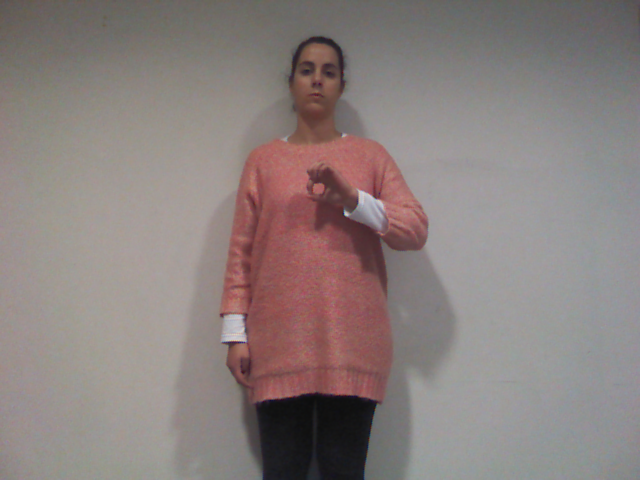
\includegraphics[interpolate=true, height=0.50\columnwidth]{ChapterFour/1_psl.png}};
            \spy on (0.05,0.23) in node [left] at (1.6,0.9);
        \end{tikzpicture}
    \end{minipage}
    \hspace{0.00mm}
    \begin{minipage}[t]{0.3\columnwidth}
        \begin{tikzpicture}[spy using outlines={circle,red,magnification=4,size=1.4cm, connect spies}]
            \node {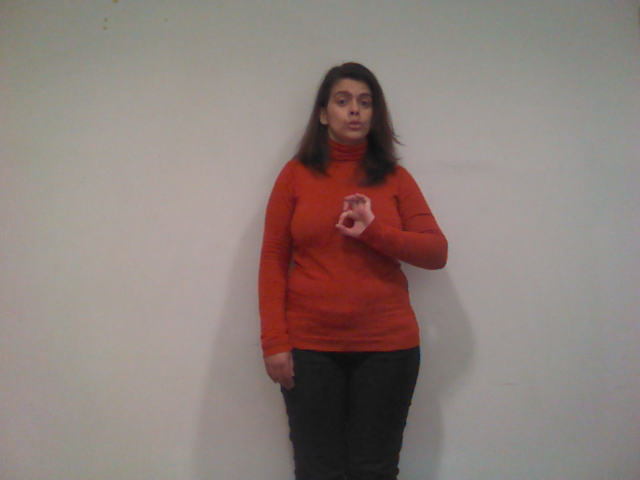
\includegraphics[interpolate=true, height=0.50\columnwidth]{ChapterFour/2_psl.png}};
            \spy on (0.16,0.07) in node [left] at (1.6,0.9);
        \end{tikzpicture}
    \end{minipage}
    \hspace{0.00mm}
    \begin{minipage}[t]{0.3\columnwidth}
        \begin{tikzpicture}[spy using outlines={circle,red,magnification=4,size=1.4cm, connect spies}]
            \node {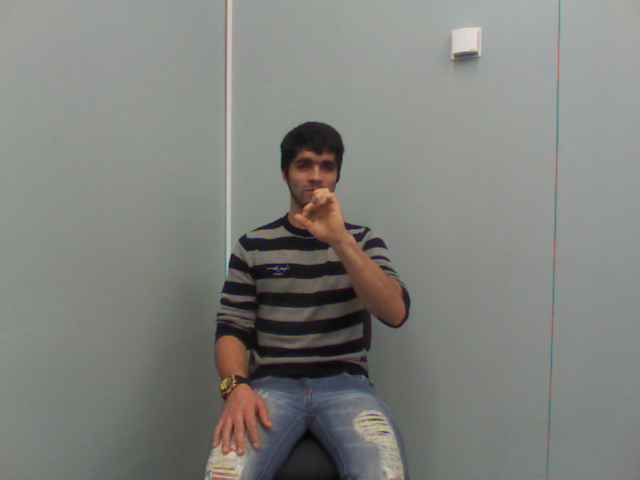
\includegraphics[interpolate=true, height=0.50\columnwidth]{ChapterFour/3_psl.png}};
            \spy on (0.02,0.08) in node [left] at (1.6,0.9);
        \end{tikzpicture}
    \end{minipage}
    \\
    \begin{minipage}[t]{0.3\columnwidth}
        \begin{tikzpicture}[spy using outlines={circle,red,magnification=4,size=1.4cm, connect spies}]
            \node {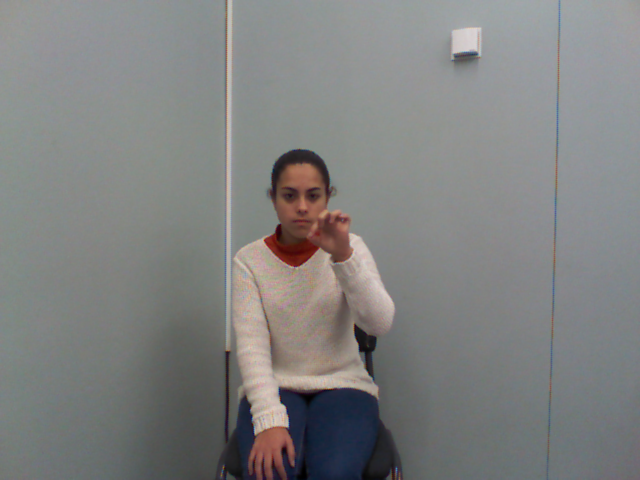
\includegraphics[interpolate=true, height=0.50\columnwidth]{ChapterFour/4_psl.png}};
            \spy on (0.04,0.05) in node [left] at (1.6,0.9);
        \end{tikzpicture}
    \end{minipage}
    \hspace{0.00mm}
    \begin{minipage}[t]{0.3\columnwidth}
        \begin{tikzpicture}[spy using outlines={circle,red,magnification=4,size=1.4cm, connect spies}]
            \node {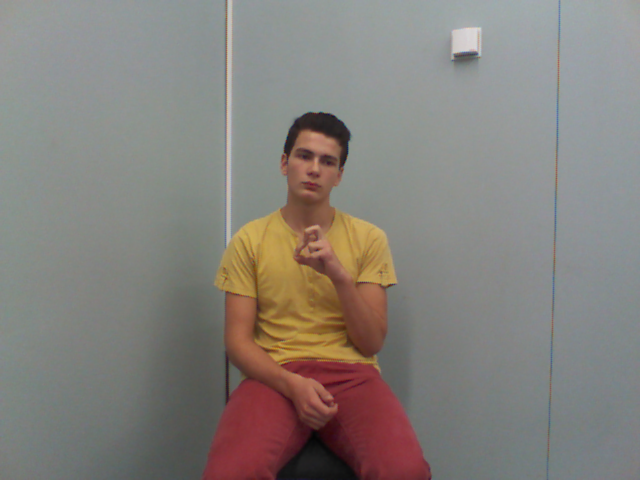
\includegraphics[interpolate=true, height=0.50\columnwidth]{ChapterFour/5_psl.png}};
            \spy on (0.001,-0.05) in node [left] at (1.6,0.9);
        \end{tikzpicture}
    \end{minipage}
    \hspace{0.00mm}
    \begin{minipage}[t]{0.3\columnwidth}
        \begin{tikzpicture}[spy using outlines={circle,red,magnification=4,size=1.4cm, connect spies}]
            \node {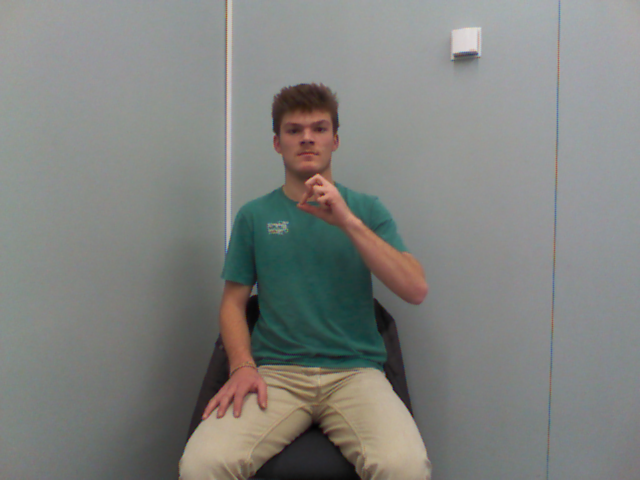
\includegraphics[interpolate=true, height=0.50\columnwidth]{ChapterFour/6_psl.png}};
            \spy on (0.02,0.17) in node [left] at (1.6,0.9);
        \end{tikzpicture}
    \end{minipage}
    \caption{Illustration of the inter-signer variability using some samples of the CorSiL database. The six signers are performing the sign ``eight" of the Portuguese sign language.}
    \label{fig:corsil}
\end{figure}

\subsubsection{Baselines}
In addition to the baselines used in \Secref{sec:adv_signer_inv_experiments} and to our previous model, we implemented two further models for comparison here:
\begin{itemize}
    \item DANN, by \citet{Ganin2015}, which we have already discussed extensively. The application of this method to our problem implied two main changes in the original method: i) the binary domain-classifier (source vs.\ target domain) was extended to $k$ classes (number of signers in the training data); ii) since our data is fully annotated (sign classes and signer identities are always available), training was performed in a fully supervised fashion.
    \item DTML, by \citet{Hu2016}, a reconstruction-based domain adaption algorithm. The implementation of this methodology for our particular task also implied the generalization of the original model from one single domain to $k$ source domains.
\end{itemize}

\subsubsection{Results and discussion}

\Tableref{tab:desire_jt_mklm_results} shows the classification accuracy of the proposed DeSIRe model and the two aforementioned baselines on Jochen-Triesch and MKLM datasets. For easy comparison, we replicate the results from \Tableref{tab:adv_signer_inv_results} for our adversarial model (\Secref{sec:adv_signer_inv}). The results for the remaining baselines are omitted since they are the same as before and inferior to those of our adversarial model.

\begin{table}[t]
    \centering
    \resizebox{\linewidth}{!}{
        \begin{tabular}{c|c c c|c c c}
            & \multicolumn{3}{c|}{Jochen Triesch} & \multicolumn{3}{c}{MKLM}\\
            & Uniform  Bg.      & Complex Bg.        & Both  & Avg. $\pm$ std.  & min         & max        \\ \hline
            DANN \cite{Ganin2015} & 98.1 & 83.8  & 93.3 & 94.3 \footnotesize{$\pm 2.5$} & 91.5 & 96.5 \\
            DTML \cite{Hu2016} & 98.8 & 85.6  & 94.4 & 94.1 \footnotesize{$\pm 3.8$} & 87.0 & 97.5 \\
            \hline
            Proposed adv.\ model (\Secref{sec:adv_signer_inv})       &      98.8     & 91.3
            &   96.3 &    94.8 \footnotesize{$\pm 3.5$}      &  89.5
            &  \textbf{100.0}    \\
            DeSIRe & \textbf{99.7} & \textbf{92.5} & \textbf{97.3} & \textbf{96.8} \footnotesize{$\pm 2.4$} & \textbf{93.0} & 99.0
    \end{tabular}}
    \caption{Classification accuracy (\%) of DeSIRe and baselines on Jochen-Triesch and MKLM datasets.}
    \label{tab:desire_jt_mklm_results}
\end{table}

A first observation is the superior performance of DeSIRe. It is also worth mentioning that our previous model for domain generalization outperformed DANN and DTML in most settings. Nevertheless, DeSIRe achieved the best overall classification accuracy in all settings. Another interesting observation is the performance of DeSIRe against complex backgrounds, which even exceeds that of our previous model. These results demonstrate the robustness of the proposed model to inter-signer variability as well as its capability of dealing with the large intra-signer variability of this dataset. As previously explained in \Secref{sec:desire_loss}, the robustness to intra-signer variability is mostly due to the proposed sampling scheme of the sign repetition introduced to the decoder network, which enforces the learned latent representations to discard this type of variability. Another important reason that may explain the superiority of DeSIRe is the fact that this model aligns class-conditional distributions, rather than marginal ones. Since all signers have labeled data and, in the datasets we use here, the marginal class distributions are balanced across signers, aligning marginal feature distributions is less problematic here than it was for domain adaptation (Chapter \ref{chp:domain_adaptation}). Anyway, the explicit alignment of conditional distributions is preferable since it promotes class clustering in the latent space. Additionally, as the encoder is conditioned on the signer identity, the feature transformation learned by DeSIRe is domain-dependent, which is not the case for the remaining models.

The classification accuracy for sign classification in the CorSiL database is presented in \Tableref{tab:desire_corsil_results}. As the SI-PSL database contains a large number of sign classes (31), the results are presented in terms of top-1, top-3 and top-5 classification accuracy. As shown in the table, DeSIRe outperformed both the implemented baselines and the state of the art domain adaption methods in all the three classification metrics. However, it should be noticed that, regardless of the employed methodology, the overall performance in this database is significantly below that obtained in the other two databases. These results attest to the difficulty of the classification task on the presented database and should encourage further research on signer-independent SLR.

\begin{table}[t]
    \centering
    \begin{tabular}{c|c c c}
            & Top-1  & Top-3 & Top-5 \\\hline
            DANN \cite{Ganin2015} & 48.7             & 75.5                    & 83.3           \\
            DTML \cite{Hu2016} & 39.3            & 68.0                    & 79.8            \\
            \hline
            CNN (baseline 1)                              & 46.0           & 74.7          & 86.8        \\
            CNN with triplet loss (baseline 2)            &  42.7          & 72.3          & 82.0       \\
            Proposed adv.\ model (\Secref{sec:adv_signer_inv}) & 49.1 & 76.0 & 85.2 \\
            DeSIRe         & \textbf{51.9}  & \textbf{76.6} & \textbf{87.9}        \\
    \end{tabular}
    \caption{Classification accuracy (\%) of DeSIRe and baselines on the CorSiL dataset.}
    \label{tab:desire_corsil_results}
\end{table}

Since DeSIRe is a rather complex model, with multiple loss terms and techniques to enhance its performance, we believe it is highly instructive to provide a more thorough analysis of its training behavior and further experimental results. Both are presented in Appendix~\ref{appendix:desire}. Specifically, we present a qualitative and quantitative analysis of the learned latent representations in Appendices \ref{sec:desire_tsne} and \ref{sec:desire_clusters}, respectively. We illustrate the interaction of the multiple loss terms in Appendix~\ref{sec:desire_training_behav}. A hyperparameter sensitivity analysis is conducted in Appendix~\ref{sec:desire_hyperparams}.

\subsection{Conclusion}
\label{sec:desire_conclusion}
The work we have just presented addresses the topic of signer-independent sign language recognition. To tackle this problem, we proposed a novel end-to-end deep neural network along with a well-designed loss function that explicitly models signer-invariant latent representations from the data. Specifically, the proposed model is composed by two main modules: i) a conditional variational autoencoder (CVAE) and ii) a classifier. The purpose of the CVAE module is to learn latent representations of the input data whose conditional posterior distribution, given the image and its sign label, is independent of the signer identity. During the training stage, the CVAE plays the role of a teacher model for the classifier, since the conditional posterior distribution over latent representations is used to regularize the hidden representations of the classifier. These signer-invariant hidden representations are then used for a robust signer-independent SLR recognition. Experimental results demonstrate the robustness of the proposed model to new test signers. The proposed model provides quite promising results, outperforming the implemented baseline methods and current state-of-the-art SLR and domain adaptation methods in different SLR databases. Extending the proposed DeSIRe model to dynamic signs (i.e.\ video) is an interesting direction for future work.


\section{Summary}
\label{sec:dg_summary}
In this chapter, we treated the problem of domain generalization. As we have seen, DG is closely related to domain adaptation, which was our focus in Chapter \ref{chp:domain_adaptation}. The main difference is the fact that in DG the target domain is not known beforehand, i.e.\ at training time, so no data from such domain is available, neither labeled nor unlabeled. The goal is then to build a model that can generalize well to new target domains, which are assumed to be fairly similar to the source ones. In practice, we have seen that most algorithms for DA can be adapted to the problem of DG with minor modifications.

Sign language recognition was the motivating application for both methods presented in this chapter. This is a problem where the DG setting fits perfectly, as an SLR automatic system should ideally perform consistently well regardless of the signer identity. For this purpose, we first presented a model in \Secref{sec:adv_signer_inv} that builds upon existing adversarial-based methods for DA and DG. The main difference is a novel definition for the adversarial objective. Instead of maximizing the discriminator loss, our adversarial routine aims to force this module to output a uniform distribution over the signer identities. This results in a smoother objective with bounded gradients, besides providing a more interpretable way to assess the signer-independence of the learned representations. In \Secref{sec:adv_iris_attack}, we showed that a very similar idea can be applied to increase the robustness of iris presentation attack detection methods to unseen attacks. Since the input data used there were not images, this experiment validated the effectiveness of the proposed adversarial model for non-visual data as well.

In \Secref{sec:desire}, we introduced another solution for the DG problem in the context of SLR, which outperforms the former and all baselines we have compared it with. Our DeSIRe model uses a variational autoencoder to learn signer-invariant representations which are used to train a non-probabilistic feature extractor. Apart from the multiple training strategies that enhance the robustness of the learned representations, the superior performance of DeSIRe is likely explained by the fact that it aligns class conditional distributions, instead of marginals, and also by the domain-dependent feature transformation learned by the encoder network.